\documentclass[12pt]{article}

\usepackage[margin=1in]{geometry}
\usepackage{amsmath,amssymb}
\usepackage{graphicx}
\graphicspath{{../output/figures/}}
\usepackage{booktabs}
\usepackage{tabularx}
\usepackage{multirow}
\usepackage{natbib}
\usepackage{setspace}
\usepackage{hyperref}
\usepackage[T1]{fontenc}
\usepackage{lmodern}

\doublespacing

\title{The Consumption Cost of Labor Informality:\\ Evidence from Russia's Self-Employment Tax Reform}
\author{Anna Malkova\thanks{Florida Institute of Technology. Email: amalkova@fit.edu.}}
\date{\today}

\begin{document}

\maketitle

\begin{abstract}
Russia's simplified self-employment tax regime (NPD) provides a tax number and a smartphone receipt app---but no sick leave, no unemployment benefits, no pension. Standard theory predicts this should not affect consumption insurance. Using panel data from the Russian Longitudinal Monitoring Survey (2010--2023), I first document that informal wage workers face nearly twice the income--consumption pass-through of formal workers ($\beta = 0.116$ vs.\ $0.064$, $p < 0.001$), despite earning comparable wages. I then exploit the NPD's staggered rollout across regions in 2019--2020 and show that the pass-through for informal wage workers drops from 0.128 to 0.068 after NPD availability---converging exactly to the formal worker level. The improvement is concentrated in informal wage workers, absent for the self-employed and formal workers, and cannot reflect reclassification: the NPD has zero effect on survey-measured informality. These results point to a \textit{legal economic identity} channel---operating through credit access and formal contracting rather than social insurance---that standard wage-based welfare measures miss entirely.

\medskip\noindent
\textbf{JEL codes:} J46, O17, D12, H26, G21

\medskip\noindent
\textbf{Keywords:} informality, consumption insurance, tax formalization, credit access, Russia, self-employment
\end{abstract}

\newpage

%% ============================================================
\section{Introduction}
\label{sec:intro}
%% ============================================================

A self-employed worker who registers for Russia's simplified tax regime---the \textit{nalog na professionalnyi dokhod} (NPD)---gains no sick leave, no unemployment benefits, no pension rights. The registration provides a tax number and a smartphone application for issuing receipts. Standard models of informality predict that this kind of formalization should have no effect on consumption insurance: in both structural frameworks \citep{Ulyssea2018} and search models \citep{Meghir2015, BoeriGaribaldi2007}, the welfare benefit of formal status operates through social insurance access or the wage premium associated with formal contracts.\footnote{See \citet{LaPortaShleifer2014} and \citet{Ulyssea2020} for surveys.} I show that it cuts the income--consumption pass-through for informal workers nearly in half.

This finding is a puzzle. It implies that there is a large consumption insurance channel of informality that operates \textit{independently of social insurance}---through what I call the legal economic identity channel. A worker with a tax registration can invoice firms that require documented suppliers, access bank credit products that demand proof of income, and operate without fear of fines for unregistered economic activity. These channels are invisible to wage-based welfare measures and absent from standard structural models, yet they appear to account for most of the consumption insurance gap between formal and informal workers.

This paper documents the puzzle in two steps. First, I establish a novel descriptive fact: informal workers in Russia face dramatically worse consumption insurance than formal workers, despite earning comparable wages. Using fourteen waves of the Russian Longitudinal Monitoring Survey (RLMS-HSE, 2010--2023) with 43,280 individuals, I apply the consumption insurance test of \citet{Townsend1994}, regressing consumption growth ($\Delta \ln c$) on income growth ($\Delta \ln w$) by employment type. The income--consumption pass-through is $\beta = 0.116$ for informal wage workers versus $\beta = 0.064$ for formal workers ($p < 0.001$ for both)---nearly twice the rate. Consumption growth variance is 12.4\% higher for informal workers (Levene's test $p = 0.001$). These differences are large, precisely estimated, and robust. They constitute, to my knowledge, the first application of the Townsend framework to the formal--informal distinction in any country.

Second, I provide suggestive causal evidence that access to formal legal status---even without social insurance---improves consumption smoothing. I exploit the staggered rollout of the NPD across Russian regions in 2019--2020 in a triple-difference design. The by-type results are striking: the income--consumption pass-through for informal wage workers drops from 0.128 pre-NPD to 0.068 post-NPD, converging exactly to the formal worker level. The formal worker pass-through is unchanged (0.059 to 0.068), as is the self-employed pass-through---the improvement is concentrated entirely in the group with the worst pre-existing insurance and the fewest alternatives to NPD. The triple-difference coefficient is $\hat{\beta}_4 = -0.042$, economically meaningful but statistically imprecise ($p = 0.25$) due to the limited number of clusters (32 oblasts) and the small informal sample ($N \approx 4{,}100$).

The puzzle is sharpened by two additional findings. First, the NPD has exactly zero effect on RLMS-measured informality ($\hat{\beta} = 0.000$, $p = 0.97$): registering for the tax app does not change how workers describe their employment in the survey. The improvement in consumption insurance is not driven by workers gaining social insurance through reclassification---it operates through other channels. Second, the effect is absent for self-employed workers, who already had access to formalization through the more burdensome individual entrepreneur (IP) status. The NPD matters specifically for informal \textit{wage} workers, for whom it represents the first accessible path to any form of legal economic identity.

What channels could explain this? I investigate three mechanisms: credit access, savings mobilization, and client contracting. Using regional variation in banking infrastructure from administrative data, I test whether the NPD's consumption insurance effect is larger in regions with greater financial development---as would be predicted if the mechanism operates through credit markets. I also examine whether savings behavior changes differentially for informal workers after NPD availability, and whether the effect scales with NPD take-up intensity across regions. These tests are suggestive rather than definitive, but they consistently point toward a credit-and-contracting channel rather than a direct insurance channel.

This paper makes three contributions. First, I document a consumption insurance cost of informality that is invisible to the wage distribution: informal and formal workers earn comparable wages, but informal workers bear nearly twice the consumption risk. The Townsend test provides a transparent welfare measure that requires neither the structural assumptions of \citet{Ulyssea2018} nor the high-frequency flow data needed by search models. Second, I present evidence---descriptive and suggestive-causal---that \textit{tax formalization alone}, without social insurance, substantially reduces this cost. This challenges the standard view that the welfare benefit of formalization operates through social insurance access, and implies that models of informality should incorporate a legal-identity channel that standard frameworks miss. Third, I contribute to the literature on Russia's informal sector \citep{GimpelsonKapeliushnikov2014, LehmannZaiceva2013} by documenting a welfare cost that is hidden from the extensive research on Russian wage inequality---and by showing that a remarkably light-touch policy intervention (a smartphone tax app) can partially close the gap.

The remainder of the paper proceeds as follows. Section~\ref{sec:literature} reviews the related literature. Section~\ref{sec:background} describes the institutional setting and the NPD reform. Section~\ref{sec:data} presents the data. Section~\ref{sec:empirical} describes the empirical strategy. Section~\ref{sec:results} presents the main results. Section~\ref{sec:mechanisms} investigates mechanisms. Section~\ref{sec:conclusion} concludes.


%% ============================================================
\section{Related Literature}
\label{sec:literature}
%% ============================================================

This paper connects three strands of literature: the welfare analysis of labor informality, the consumption insurance and risk-sharing literature, and research on tax simplification and formalization.

\subsection{Welfare costs of informality}

The question of how much informality costs workers and the economy has produced two dominant methodological approaches. The first is the structural firm-side tradition, exemplified by \citet{Ulyssea2018}, which models firms' decisions to operate formally or informally given enforcement intensity and registration costs. In this framework, welfare is measured through aggregate productivity: informality is costly because it prevents efficient reallocation and keeps unproductive firms alive. \citet{Meghir2015} embed informality in a labor search model with firm heterogeneity, where welfare costs arise from misallocation across formal and informal jobs. These models provide valuable insights into the aggregate consequences of informality but are silent on the household-level consumption smoothing channel. A firm that formalizes may raise aggregate TFP, but the welfare gain to the worker depends on whether formalization also improves access to insurance---a margin these models do not capture.

The second approach uses search-and-matching models with formal and informal sectors \citep{BoeriGaribaldi2007, CharlotMalherbet2013, BoschEstebanPretel2012}. Workers transition between formal employment, informal employment, and unemployment; welfare in each state is determined by the wage and the probability of transitioning to other states. The welfare cost of informality in these models is the wage gap plus the option value of formal employment (lower separation risk, access to unemployment insurance). While closer to the insurance channel I emphasize, these models still measure welfare through wages and transition probabilities rather than observed consumption outcomes. Moreover, they assume informality arises from search frictions rather than voluntary choice---an assumption that fits Russia poorly, where many informal self-employed workers report choosing informality over formal wage employment \citep{Maloney2004}.

\citet{Ulyssea2020} provides a comprehensive survey and concludes that enforcement on the extensive margin (whether firms register at all) is the most effective policy lever. My findings complement this by showing that even when informality does not change on the extensive margin---the NPD has no effect on RLMS-measured informality rates---access to a simplified formal channel can improve consumption insurance for workers who remain in the informal sector by their own survey responses.

A separate literature uses reduced-form approaches to estimate the costs of informality to workers. \citet{Perry2007} and \citet{Levy2008} emphasize the ``exclusion'' view---informality as involuntary, driven by barriers to formal employment---versus the ``exit'' view of \citet{Maloney2004}, where informality represents a rational choice given the cost-benefit calculus of formalization. \citet{LaPortaShleifer2014} argue for a dual-economy model where informal firms are fundamentally different from formal firms, neither competing with them nor transitioning into formality. My approach is agnostic on this debate: regardless of why workers are informal, I measure the consumption consequence of lacking social insurance coverage.

\subsection{Consumption insurance and risk sharing}

The Townsend village economy framework \citep{Townsend1994} provides the theoretical foundation for my welfare measure. Under full risk sharing, idiosyncratic income shocks should not affect individual consumption---only aggregate village-level shocks should matter. The pass-through coefficient $\beta$ in a regression of consumption growth on income growth measures the degree to which this insurance benchmark is violated. \citet{Townsend1994} rejects full insurance in Indian villages but finds substantial smoothing; subsequent work has applied this framework to a wide range of settings \citep{Cochrane1991, Mace1991, Attanasio2002}.

\citet{Morduch1995} distinguishes between \textit{income smoothing} (ex ante strategies to reduce income risk) and \textit{consumption smoothing} (ex post mechanisms to buffer consumption from realized income shocks). Informal workers may engage in income smoothing through portfolio diversification but have limited access to the consumption smoothing mechanisms that formal institutions provide. My findings confirm this asymmetry: self-employed workers, who have the most income-smoothing options, show lower consumption variance than informal wage workers despite both lacking formal social insurance.

The consumption insurance framework has been applied to study the welfare effects of specific institutions. \citet{Gertler2002} show that Indonesian households cannot fully insure against major illness; \citet{Genoni2012} finds that informal risk-sharing networks provide partial but incomplete insurance in rural Colombia. To my knowledge, this paper is the first to apply the Townsend framework specifically to the formal--informal distinction in a transition economy.

\subsection{Tax simplification and formalization}

A growing literature studies whether simplifying tax and registration requirements induces formalization. \citet{Monteiro2012} study Brazil's SIMPLES program, which reduced tax and regulatory costs for small firms, and find increased formalization and revenue growth. \citet{Bruhn2011} exploits a Mexican reform that simplified business registration and finds modest increases in formal firm registration. \citet{deMelMcKenzieWoodruff2013} provide experimental evidence from Sri Lanka, showing that the majority of informal firms do not formalize even when offered substantial monetary incentives, but those that do see increased profits and access to formal credit.

Russia's NPD regime represents an unusually clean natural experiment in this literature for several reasons. First, the staggered rollout across regions provides temporal and geographic variation in treatment. Second, the reform dramatically reduced compliance costs: registration through a mobile application, no accounting requirements, and a flat 4--6\% tax rate on gross revenue. Third, the reform was federal legislation implemented uniformly within each region, reducing concerns about endogenous adoption. The NPD attracted over 15 million registrants by early 2026, suggesting substantial take-up.

\subsection{Informality in Russia}

Russia presents a distinctive setting for studying informality. The informal sector is large---estimated at 20--30\% of employment depending on the definition \citep{GimpelsonKapeliushnikov2014}---and remarkably stable over time. Unlike Latin American countries where informality is concentrated in low-productivity services and agriculture, Russian informality spans construction, trade, transportation, and professional services. \citet{LehmannZaiceva2013} document substantial regional variation, from approximately 5\% in Moscow to nearly 40\% in the North Caucasus.

A distinctive feature of Russian informality is the prevalence of ``envelope wages''---formal employment where a portion of compensation is paid off the books to avoid social insurance contributions \citep{GimpelsonKapeliushnikov2014}. In the RLMS, approximately 12\% of wage workers report that their wages are not fully officially registered. This intensive-margin informality means that even workers classified as formally employed may have partial exposure to the insurance gap I document.

The institutional context is also unusual in that Russia provides universal access to a basic public healthcare system and maintains a flat-rate pension system, potentially attenuating the insurance value of formal employment relative to countries where all social benefits are tied to formal employment status. My finding that informal workers nonetheless face significantly worse consumption insurance suggests that the social insurance channel operates even in this relatively egalitarian institutional setting.


%% ============================================================
\section{Institutional Background: The NPD Reform}
\label{sec:background}
%% ============================================================

This section describes the institutional setting for self-employment in Russia and the NPD reform that provides the identifying variation for my empirical analysis.

\subsection{Self-employment before the NPD}

Prior to 2019, workers in Russia who wished to operate legally outside of standard wage employment had two main options. The first was to register as an \textit{individualnyi predprinimatel} (IP, ``individual entrepreneur'').\footnote{Federal Law No.~129-FZ ``On State Registration of Legal Entities and Individual Entrepreneurs,'' August 8, 2001.} IP status required registration with the Federal Tax Service, opening a business bank account, maintaining accounting records, filing quarterly tax returns, and paying mandatory social insurance contributions (pension fund and compulsory medical insurance) regardless of whether the entrepreneur earned any income. In 2018, the minimum annual social insurance payment for an IP was approximately 32,400 rubles (roughly \$500 at the time), rising with income above 300,000 rubles. IP registrants could choose among several tax regimes---the simplified taxation system (\textit{uproshchonnaya sistema nalogooblozheniya}, USN), the imputed income system (ENVD), or the patent system (\textit{patentnaya sistema nalogooblozheniya}, PSN)---each with its own rates, thresholds, and reporting requirements.

The second option was the patent system, available since 2013 for certain enumerated activities (tutoring, cleaning, minor repairs, etc.). The patent allowed an individual to pay a fixed annual fee in lieu of income taxes and social contributions, but coverage was limited to a narrow list of occupations specified by regional legislation, and the worker still needed to register as an IP.

The complexity and fixed costs of IP registration created a substantial barrier to formalization for small-scale self-employed workers. A freelance translator, a taxi driver, or a construction worker earning modest and irregular income faced the same accounting and social insurance obligations as a business owner with employees and substantial revenue. For many, the cost-benefit calculus favored remaining informal---operating without registration, receiving payment in cash, and avoiding both taxes and the bureaucratic burden of IP status \citep{Maloney2004, Perry2007}.

\subsection{The NPD regime}

On November 27, 2018, President Putin signed Federal Law No.~422-FZ ``On the Conduct of an Experiment to Establish a Special Tax Regime `Tax on Professional Income'\thinspace'' (\textit{nalog na professionalnyi dokhod}, NPD). The law created a new tax status---\textit{samozanyatyi} (``self-employed'')---that was explicitly designed to lower the barrier to formalization for individuals earning income outside of standard employment contracts.

The NPD regime has several distinctive features:

\begin{enumerate}
\item \textbf{Low tax rates.} The NPD tax rate is 4\% on income received from individuals and 6\% on income from legal entities, applied to gross revenue with no deductions. By comparison, IP registrants under the simplified system paid 6\% on revenue or 15\% on profit, plus mandatory social insurance contributions.

\item \textbf{No social insurance contributions.} NPD registrants are exempt from mandatory pension and medical insurance contributions. This is the feature most consequential for my analysis: NPD status provides legal formalization---an official tax registration and the ability to issue receipts to clients---without providing access to social insurance. In principle, NPD registrants can make voluntary pension contributions, but take-up of this option has been minimal.

\item \textbf{Minimal compliance costs.} Registration is conducted entirely through a mobile application (``Moy Nalog,'' or ``My Tax''), developed by the Federal Tax Service. The application allows registrants to issue electronic receipts, track income, and pay taxes---all from a smartphone. There are no accounting requirements, no quarterly filings, and no need to open a business bank account. Tax is calculated automatically by the application and paid monthly.

\item \textbf{Revenue cap.} Annual income under the NPD cannot exceed 2.4 million rubles (approximately \$30,000--40,000 depending on the exchange rate). Workers exceeding this threshold must register as IP or form a legal entity.

\item \textbf{Restrictions.} NPD registrants cannot hire employees, resell goods (as opposed to selling goods of their own production), or engage in certain regulated activities. The regime is available to both Russian citizens and citizens of EAEU member states.
\end{enumerate}

\noindent The NPD thus occupies a distinctive position in the formalization landscape: it provides \textit{tax formalization} (legal registration, receipt issuance, tax compliance) without providing \textit{labor formalization} (social insurance, pension accrual, sick leave, unemployment benefits). This distinction is central to interpreting my results: the NPD does not directly improve social insurance coverage for informal workers, but it may affect consumption smoothing through indirect channels---access to formal credit markets, the ability to contract with firms that require documented suppliers, reduced risk of fines for unregistered activity, and the psychological security of legal status.

\subsection{Staggered rollout}

The NPD was introduced as a ``tax experiment'' with a staggered regional rollout, providing the geographic and temporal variation that I exploit for identification. The rollout proceeded in three main waves:

\begin{itemize}
\item \textbf{Wave 1 (January 1, 2019):} Four pilot regions---Moscow, Moscow Oblast, Kaluga Oblast, and the Republic of Tatarstan. These regions were chosen for their economic size (Moscow), geographic proximity to the capital (Moscow Oblast, Kaluga), and administrative capacity (Tatarstan).

\item \textbf{Wave 2 (January 1, 2020):} Nineteen additional regions, including St.~Petersburg, major Ural and Siberian cities (Sverdlovsk, Chelyabinsk, Novosibirsk, Omsk), southern Russia (Rostov, Volgograd, Voronezh), and the oil-producing autonomous okrugs (Khanty-Mansiysk, Yamalo-Nenets). Federal Law No.~428-FZ of December 15, 2019, authorized this expansion.

\item \textbf{Wave 3 (July--October 2020):} All remaining regions joined between July 1 and October 19, 2020, authorized by Federal Law No.~101-FZ of April 1, 2020. The bulk of regions (approximately 50) joined on July 1; a handful joined on later dates through October, with the Republic of Ingushetia being the last to adopt on October 19.
\end{itemize}

\noindent The staggered adoption was determined by federal legislation, not by regional governments' choices, which mitigates the concern that regions selected into early adoption based on local labor market conditions.\footnote{The pilot regions were selected by the federal Ministry of Finance based on administrative readiness and economic scale, not on informality rates or labor market outcomes. Tatarstan, for example, was chosen because of its track record as a testing ground for federal digital government initiatives.} The expansion in 2020 was accelerated relative to the original plan in part due to the COVID-19 pandemic: the government viewed NPD registration as a way to provide a legal framework for workers displaced from formal employment during lockdowns.

\subsection{Take-up}

Take-up of the NPD has been substantial and rapid. The Federal Tax Service reports that the number of NPD registrants grew from approximately 340,000 at the end of 2019 (after one year in four regions) to 1.6 million by the end of 2020 (after nationwide expansion), 3.9 million by the end of 2021, and over 10 million by the end of 2023. By early 2026, the cumulative number of NPD registrants exceeded 15 million---approximately 20\% of the total employed population, though many registrants are part-time or occasional users.

Moscow accounts for a disproportionate share: approximately 2.3 million registrants, or 15\% of the national total. The geographic concentration reflects both the large informal economy in Moscow's service sector and the higher awareness of the digital registration platform. Outside of Moscow, take-up has been highest in regions with large urban service economies (St.~Petersburg, Krasnodar, Sverdlovsk) and lower in predominantly rural or industrial regions.

Several features of the NPD take-up pattern are relevant for my analysis. First, the scale of registration suggests that the reform reached a substantial fraction of the informally employed population, not just a marginal group. Second, many NPD registrants appear to be workers who were previously operating informally rather than workers transitioning from IP status: the number of IP registrations did not decline after NPD introduction, suggesting limited substitution.\footnote{Rosstat data show that the number of registered individual entrepreneurs remained approximately stable at 3.7--3.9 million between 2018 and 2023.} Third, the NPD was taken up by workers in precisely the occupations that dominate informal employment in the RLMS---taxi driving, tutoring, domestic services, freelance IT work, and small-scale trade.

\subsection{Implications for identification}

The staggered rollout of the NPD creates variation across regions and time in access to a simplified formalization channel. My identification strategy exploits this variation in a difference-in-differences framework, comparing the consumption insurance gap between informal and formal workers in regions that have adopted the NPD versus regions that have not yet adopted it.

Two features of the reform are important for interpreting the results. First, because the NPD provides tax formalization \textit{without} social insurance, any improvement in consumption smoothing must operate through indirect channels rather than through direct access to unemployment benefits or sick leave. This makes the NPD a conservative test of the formalization channel: if even tax-only formalization improves consumption insurance, the welfare gains from full labor formalization (with social insurance) are likely larger. Second, the NPD does not change the employment status of workers as measured by the RLMS survey questions about official employment and contracts. A worker who registers as \textit{samozanyatyi} under the NPD will still report in the RLMS that they do not have an official labor contract (\textit{trudovoi dogovor}). This means the NPD cannot mechanically reclassify workers from informal to formal in my data; any changes in the consumption insurance gap reflect genuine behavioral responses rather than measurement artifacts.


%% ============================================================
\section{Data}
\label{sec:data}
%% ============================================================

I use individual-level panel data from the Russia Longitudinal Monitoring Survey---Higher School of Economics (RLMS-HSE), merged with household-level consumption data and the regional NPD rollout schedule.

\subsection{The RLMS-HSE}

The RLMS-HSE is an annual nationally representative panel survey conducted since 1994, based on a multi-stage probability sample of residential addresses across the Russian Federation.\footnote{The RLMS-HSE is conducted by the National Research University Higher School of Economics and ZAO Demoscope, with the participation of the Population Center at the University of North Carolina at Chapel Hill and the Institute of Sociology of the Federal Center of Theoretical and Applied Sociology of the Russian Academy of Sciences. Data are available at \url{https://www.hse.ru/rlms/}.} The survey interviews all adult members of selected households, collecting detailed information on employment, income, health, and demographic characteristics at the individual level, and on expenditures, assets, and housing at the household level. I use waves 19 through 32, corresponding to survey years 2010--2023, which provide four pre-NPD periods (2010--2013) before Russia's 2014 macroeconomic shock, a full pre-period (2010--2018), and five post-NPD years (2019--2023).

The raw data contain 268,085 individual-year observations covering 43,280 unique individuals in 13,765 households across 32 federal subjects (oblasts). Not all individuals appear in every year: panel attrition and household replacement produce an unbalanced panel, with approximately 18,000--22,000 individuals observed per wave.

\subsection{Employment and informality classification}

I classify employment status using the individual-level questionnaire. Workers are first identified as employed based on a direct question (RLMS variable \texttt{j1}: ``Did you work in the last 30 days?''). Among the employed, I distinguish three groups:

\begin{enumerate}
\item \textbf{Formal wage workers} are employees (not self-employed, \texttt{j4\_1} $\notin \{4, 5\}$) who report that their employment is officially registered (\texttt{j11\_1} = 1, indicating that the employer has registered the employment relationship with the relevant authorities and the worker has an official labor contract, \textit{trudovoi dogovor}).

\item \textbf{Informal wage workers} are employees who report that their employment is \textit{not} officially registered (\texttt{j11\_1} = 2). These workers lack a formal labor contract and are therefore excluded from employer-provided social insurance contributions (pension, social insurance fund, compulsory medical insurance).

\item \textbf{Self-employed workers} are those who report their primary activity as self-employment or own business (\texttt{j4\_1} $\in \{4, 5\}$), regardless of their registration status.
\end{enumerate}

In addition to this primary classification, I construct two supplementary informality indicators. The first is an ``envelope wages'' measure based on the question ``What share of your wages is officially registered?'' (\texttt{j10\_1}): workers reporting less than 100\% official wages are classified as having envelope wages. Approximately 12\% of wage workers in the sample report partial off-the-books payment. The second is a composite informality indicator that takes the value one if a worker has either no official contract \textit{or} envelope wages. This composite measure captures both the extensive margin (entirely unregistered employment) and the intensive margin (formally employed but with partially informal compensation).

Table~\ref{tab:summary_emptype} reports summary statistics by employment type. Among the employed, formal wage workers account for approximately 86\% of observations, informal wage workers for 7\%, and self-employed workers for 7\%. The three groups are broadly similar in mean wages---formal workers earn 25,900 rubles per month, informal wage workers 22,500 rubles, and self-employed workers 33,400 rubles---but differ in composition: informal wage workers are younger (mean age 39.6 vs.\ 41.8 for formal) and more likely to be male (57\% vs.\ 45\%). Self-employed workers are disproportionately male (74\%) and report the highest mean wages, consistent with the ``exit'' view of informality as a voluntary choice for higher-earning workers \citep{Maloney2004, Perry2007}.

\subsection{Consumption}

Consumption is measured at the household level and matched to individuals through the household identifier (\texttt{id\_h}). All members of the same household share the same consumption observation in a given year. I construct a monthly consumption aggregate from three components:

\begin{itemize}
\item \textbf{Food expenditure}: ``How much did your family spend on food in the last 30 days?'' (\texttt{e4}). This is the largest component, averaging 15,100 rubles per month.

\item \textbf{Clothing expenditure}: The sum of adult (\texttt{e6\_1}) and child (\texttt{e6\_2}) clothing and footwear expenditures over the past three months, divided by three to convert to a monthly equivalent. This averages 5,000 rubles per month.\footnote{The RLMS questionnaire includes a filter question (\texttt{e5}: ``Did your family buy clothing or shoes in the last 3 months?''); the expenditure question is asked only of households answering yes. A separate variable \texttt{e6} that was intended to capture total clothing expenditure is empty in all waves from 2010 onward, so I use the adult and child subcategories.}

\item \textbf{Utility expenditure}: Rent and utility payments in the last 30 days (\texttt{e11}), averaging 4,600 rubles per month.\footnote{The survey includes a filter question (\texttt{e10}: ``Did your household pay for rent or utilities in the last 30 days?''); \texttt{e11} records the amount for those who answer yes.}
\end{itemize}

\noindent Total monthly consumption is the sum of these three components, requiring at least one non-missing component.\footnote{Mean total consumption rises from approximately 14,000 rubles per month in 2010 to 35,000 rubles by 2023, reflecting both real growth and inflation. All consumption figures are in nominal rubles; the key outcome variable---consumption \textit{growth}---differences out common price changes within a household over time.} I take the natural logarithm and compute consumption growth as $\Delta \ln c_{it} = \ln c_{it} - \ln c_{it-1}$ within individuals over consecutive survey waves. The mean consumption growth is 0.074, with a standard deviation of 0.553.

This consumption measure has two limitations. First, it omits durable goods, health expenditures, and education spending, which may respond differently to income shocks. I use a narrow measure to avoid components that are lumpy or infrequently purchased, which would add noise to annual consumption growth. Second, the measure is at the household level, not the individual level. To the extent that household members pool consumption, this is the correct unit; but it means that an informal worker's consumption growth reflects the insurance provided by the entire household, including any formally employed members.

\subsection{Income}

Income is measured as the individual's monthly wage after taxes (\texttt{j10}: ``How much money did you receive for your work in the last 30 days, after taxes?''). For wage workers, this captures take-home pay from the primary job. For self-employed workers, the variable captures self-reported earnings, which may understate true income.\footnote{The wage variable is top-coded at RLMS missing codes ($\geq$99,999,990 rubles) which I replace with missing values. After cleaning, wages range from 30 to 750,000 rubles per month, with a mean of 25,900 rubles.} I compute income growth as $\Delta \ln w_{it} = \ln w_{it} - \ln w_{it-1}$ within individuals. Mean income growth is 0.096 (SD = 0.498). The Townsend insurance test requires both consumption growth and income growth to be non-missing; the estimation sample for the main specifications contains 73,435 observations with both variables.

\subsection{Geographic matching and NPD treatment}

The RLMS identifies household location through Primary Sampling Units (PSUs), which correspond to specific cities and settlements. I match PSUs to federal subjects (oblasts) using the four-digit Goskomstat territorial codes (\texttt{ter}) from the RLMS public-use site file.\footnote{The site file maps 39 PSUs to 33 federal subjects, covering all 8 RLMS broad geographic regions.} All 268,085 observations match to an oblast, and all oblasts match to an NPD rollout date through a crosswalk between the Goskomstat codes and the region names in the NPD legislation.

I construct a binary treatment indicator $\text{post\_NPD}_{rt}$ equal to one if region $r$'s NPD start date falls in year $t$ or earlier. In the RLMS sample, the 32 oblasts map to two effective NPD cohorts: an early cohort of 4 oblasts (Moscow, Moscow Oblast, Kaluga, Tatarstan) treated from 2019, and a late cohort of 28 oblasts treated from 2020.\footnote{Although the national rollout had eight distinct adoption dates between January 2019 and October 2020, the RLMS covers only 32 of 85 federal subjects. These 32 oblasts fall into just two effective cohorts when mapped to annual survey data.} Approximately 73,000 observations (27\% of the panel) fall in the post-NPD period.

\subsection{Summary statistics}

Table~\ref{tab:summary_full} presents summary statistics for the full sample. The mean age is 38.9 years and 56\% of respondents are female, reflecting the RLMS's coverage of all household members including children and retirees. The employment rate is 43\%, consistent with the inclusion of children, students, and pensioners in the denominator. Among the employed, 15\% are classified as informal by the composite measure, with 7\% lacking an official contract and 12\% reporting envelope wages.

\begin{table}[htbp]
\centering
\caption{Summary Statistics: Full Sample}
\label{tab:summary_full}
\small
\begin{tabular}{lrrrrr}
\toprule
Variable & $N$ & Mean & Std & Median \\
\midrule
\multicolumn{5}{l}{\textit{Demographics}} \\
Age & 268,085 & 38.89 & 22.54 & 38.00 \\
Female & 268,085 & 0.563 & 0.496 & 1.00 \\
Employed & 268,085 & 0.431 & 0.495 & 0.00 \\
\\
\multicolumn{5}{l}{\textit{Employment (among employed)}} \\
Monthly wage (RUB) & 111,474 & 25,854 & 22,004 & 20,000 \\
Informal (composite) & 114,747 & 0.152 & 0.359 & 0.00 \\
No official contract & 108,558 & 0.067 & 0.251 & 0.00 \\
Has envelope wages & 97,073 & 0.120 & 0.325 & 0.00 \\
Small firm ($\leq$5 employees) & 77,681 & 0.088 & 0.284 & 0.00 \\
\\
\multicolumn{5}{l}{\textit{Consumption (household-level, monthly)}} \\
Total consumption (RUB) & 266,589 & 22,353 & 16,361 & 18,933 \\
Food expenditure (RUB) & 250,767 & 15,134 & 11,879 & 12,000 \\
Clothing expenditure (RUB) & 201,766 & 5,013 & 5,571 & 3,333 \\
Utility expenditure (RUB) & 249,151 & 4,625 & 3,852 & 4,000 \\
\\
\multicolumn{5}{l}{\textit{Growth rates}} \\
$\Delta \ln c$ & 222,629 & 0.074 & 0.553 & 0.071 \\
$\Delta \ln w$ & 82,524 & 0.096 & 0.498 & 0.057 \\
Saved money (share) & 264,755 & 0.147 & 0.354 & 0.00 \\
\bottomrule
\end{tabular}
\begin{minipage}{0.9\textwidth}
\vspace{0.3em}
\footnotesize \textit{Notes:} RLMS-HSE waves 19--32 (2010--2023). 268,085 individual-year observations, 43,280 unique individuals, 13,765 households, 32 federal subjects. Consumption is household-level (shared within household). Wages are individual after-tax monthly earnings. Informality indicators are among employed workers only.
\end{minipage}
\end{table}

\begin{table}[htbp]
\centering
\caption{Summary Statistics by Employment Type (Employed Workers)}
\label{tab:summary_emptype}
\small
\begin{tabular}{l*{3}{rr}}
\toprule
 & \multicolumn{2}{c}{Formal wage} & \multicolumn{2}{c}{Informal wage} & \multicolumn{2}{c}{Self-employed} \\
\cmidrule(lr){2-3} \cmidrule(lr){4-5} \cmidrule(lr){6-7}
Variable & Mean & Std & Mean & Std & Mean & Std \\
\midrule
Observations & \multicolumn{2}{c}{90,037} & \multicolumn{2}{c}{7,115} & \multicolumn{2}{c}{7,114} \\
\\
Monthly wage (RUB) & 25,896 & 21,544 & 22,524 & 19,006 & 33,448 & 26,451 \\
Total consumption (RUB) & 23,547 & 17,415 & 23,112 & 15,827 & 24,377 & 15,802 \\
$\Delta \ln c$ & 0.079 & 0.530 & 0.084 & 0.562 & 0.073 & 0.520 \\
$\Delta \ln w$ & 0.108 & 0.446 & 0.100 & 0.521 & 0.106 & 0.438 \\
Age & 41.76 & 12.12 & 39.65 & 13.25 & 40.42 & 11.05 \\
Female & 0.550 & 0.497 & 0.434 & 0.496 & 0.256 & 0.437 \\
\bottomrule
\end{tabular}
\begin{minipage}{0.9\textwidth}
\vspace{0.3em}
\footnotesize \textit{Notes:} Sample restricted to employed workers with non-missing employment type classification. Formal wage workers have an officially registered labor contract ($j11\_1 = 1$). Informal wage workers lack an official contract ($j11\_1 = 2$). Self-employed workers report self-employment or own business as primary activity ($j4\_1 \in \{4, 5\}$).
\end{minipage}
\end{table}


%% ============================================================
\section{Empirical Strategy}
\label{sec:empirical}
%% ============================================================

This section presents the empirical framework in three parts: the consumption insurance test that provides the welfare measure, the difference-in-differences design that identifies the effect of NPD availability, and a discussion of identification assumptions and threats.

\subsection{Consumption insurance test}

My welfare measure builds on the consumption insurance framework of \citet{Townsend1994}. Under full risk sharing---whether through formal insurance, informal networks, or complete credit markets---idiosyncratic income shocks should not pass through to individual consumption. Only aggregate shocks should matter. The degree to which this benchmark is violated provides a transparent measure of insurance failure.

Following the standard approach \citep{Cochrane1991, Mace1991, Townsend1994}, I regress individual consumption growth on individual income growth:
\begin{equation}\label{eq:townsend}
\Delta \ln c_{it} = \alpha + \beta \, \Delta \ln w_{it} + \gamma_t + \varepsilon_{it},
\end{equation}
where $\Delta \ln c_{it} = \ln c_{it} - \ln c_{it-1}$ is the change in log household consumption for individual $i$ between adjacent survey waves, $\Delta \ln w_{it}$ is the change in log individual wages, and $\gamma_t$ are year fixed effects that absorb aggregate shocks common to all workers. The first-differenced specification eliminates time-invariant individual heterogeneity (individual fixed effects).

The coefficient $\beta$ is the income--consumption pass-through and serves as my primary welfare measure. Under full insurance, $\beta = 0$: consumption is completely insulated from idiosyncratic income fluctuations. Under no insurance (autarky), $\beta = 1$: every ruble of income change translates one-for-one into consumption. Intermediate values indicate partial insurance, with higher $\beta$ corresponding to worse insurance and greater welfare loss from income volatility.

I estimate equation~(\ref{eq:townsend}) separately by employment type---formal wage, informal wage, and self-employed---to document the cross-sectional insurance gap. The key prediction is that informal wage workers, who lack access to employer-provided social insurance (sick leave, unemployment benefits, pension contributions), will exhibit a higher pass-through coefficient than formal workers.

\subsection{Difference-in-differences: the NPD natural experiment}

To move beyond cross-sectional comparisons, I exploit the staggered regional rollout of the NPD regime described in Section~\ref{sec:background}. The identifying variation comes from differences in the timing of NPD availability across regions: some oblasts gained access to the simplified self-employment regime in 2019, others in 2020. I use this variation in a difference-in-differences framework to test whether NPD availability improves consumption insurance for informal workers.

\subsubsection{Triple-difference specification}

My main specification embeds the Townsend test in a triple-difference framework:
\begin{align}\label{eq:did}
\Delta \ln c_{it} = {} & \beta_1 \, \Delta \ln w_{it} + \beta_2 \, \Delta \ln w_{it} \times \text{informal}_{it} + \beta_3 \, \Delta \ln w_{it} \times \text{post}_{rt} \nonumber \\
& + \beta_4 \, \Delta \ln w_{it} \times \text{informal}_{it} \times \text{post}_{rt} \nonumber \\
& + \delta_1 \, \text{informal}_{it} + \delta_2 \, \text{post}_{rt} + \delta_3 \, \text{informal}_{it} \times \text{post}_{rt} + \gamma_t + \varepsilon_{it},
\end{align}
where $\text{informal}_{it}$ is an indicator for informal employment (informal wage or self-employed), and $\text{post}_{rt}$ indicates that region $r$ has adopted the NPD by year $t$.

The coefficients have the following interpretation:
\begin{itemize}
\item $\beta_1$: income--consumption pass-through for formal workers in regions that have not yet adopted the NPD (the baseline insurance level);
\item $\beta_2$: the additional pass-through for informal workers relative to formal workers, pre-NPD (the informality insurance gap);
\item $\beta_3$: the change in pass-through for formal workers after NPD adoption (a placebo---NPD should not affect formal workers' insurance);
\item $\beta_4$: \textbf{the key coefficient}---the differential change in pass-through for informal workers after NPD adoption, relative to formal workers. A negative $\beta_4$ means NPD reduces the insurance gap, improving consumption smoothing for informal workers.
\end{itemize}

The ``triple difference'' arises because $\beta_4$ differences across three dimensions: (i) income growth versus no income growth (the Townsend test), (ii) informal versus formal workers, and (iii) post-NPD versus pre-NPD periods. This specification controls for any level differences in consumption between informal and formal workers ($\delta_1$), any common time trends ($\delta_2$, $\gamma_t$), and any direct effect of NPD on the consumption \textit{level} of informal workers ($\delta_3$). What $\beta_4$ captures is whether the \textit{sensitivity} of consumption to income shocks changes differentially for informal workers after NPD adoption.

Standard errors are clustered at the oblast level (32 clusters) to account for within-region correlation in both treatment assignment and outcomes.\footnote{Clustering at the oblast level is the natural choice because NPD adoption varies at the regional level. With 32 clusters, I use standard cluster-robust variance estimation. \citet{CallawayS2021} and \citet{SunAbraham2021} recommend alternative estimators for staggered designs; I discuss these in Section~\ref{sec:results}.}

\subsubsection{By-type specification}

As a complement to the triple-difference, I estimate the Townsend test separately for each employment type, interacting income growth with a post-NPD indicator:
\begin{equation}\label{eq:bytype}
\Delta \ln c_{it} = \alpha + \beta^{\text{pre}} \, \Delta \ln w_{it} + \beta^{\Delta} \, \Delta \ln w_{it} \times \text{post}_{rt} + \delta \, \text{post}_{rt} + \gamma_t + \varepsilon_{it},
\end{equation}
estimated separately for formal wage workers, informal wage workers, and self-employed workers. This yields a pre-NPD pass-through ($\beta^{\text{pre}}$) and a post-NPD pass-through ($\beta^{\text{pre}} + \beta^{\Delta}$) for each group. The prediction is that $\beta^{\Delta}$ should be negative and large for informal wage workers (whose insurance improves) and approximately zero for formal workers (whose insurance is unaffected by NPD).

\subsubsection{Event study}

To examine the dynamics of the treatment effect and test for pre-trends, I estimate the Townsend pass-through coefficient separately for each event-time year relative to NPD adoption:
\begin{equation}\label{eq:eventstudy}
\Delta \ln c_{it} = \alpha + \beta_k \, \Delta \ln w_{it} + \gamma_t + \varepsilon_{it}, \quad \text{for each } k = t - t^*_r \in \{-5, \ldots, +4\},
\end{equation}
where $t^*_r$ is the year of NPD adoption in region $r$, and the regression is estimated separately for formal and informal workers within each event-time bin. Under the identifying assumptions, the gap between the informal and formal pass-through coefficients should be stable in the pre-period (parallel pre-trends) and narrow after NPD adoption.

\subsubsection{Variance specification}

As an alternative welfare measure, I examine whether NPD reduces the variance of consumption growth for informal workers. I regress squared consumption growth on the interaction of informality and post-NPD status:
\begin{equation}\label{eq:variance}
(\Delta \ln c_{it})^2 = \delta_1 \, \text{informal}_{it} + \delta_2 \, \text{post}_{rt} + \delta_3 \, \text{informal}_{it} \times \text{post}_{rt} + \gamma_t + \varepsilon_{it},
\end{equation}
where a negative $\delta_3$ indicates that NPD reduces consumption volatility for informal workers. This specification tests whether the second moment of consumption growth---the variance---changes differentially, rather than the conditional mean relationship captured by the Townsend test.

\subsubsection{Informality rate specification}

I also test directly whether NPD changes the RLMS-measured informality rate using an individual fixed effects model:
\begin{equation}\label{eq:informality}
\text{informal}_{it} = \alpha_i + \gamma_t + \beta \, \text{post}_{rt} + \varepsilon_{it},
\end{equation}
with individual and year fixed effects and standard errors clustered at the oblast level. As discussed in Section~\ref{sec:background}, the NPD creates a tax registration status (\textit{samozanyatyi}) that does not map onto the RLMS survey-based informality definition (no labor contract, envelope wages). I therefore expect $\beta \approx 0$ in this specification. This null result is informative: it means that any changes in consumption insurance cannot be attributed to mechanical reclassification of workers from informal to formal.

\subsubsection{Worker fixed effects}

A key concern with the cross-sectional comparison is that informal workers differ from formal workers in age, gender, sector, and unobservables. While the first-differenced specification in equation~(\ref{eq:townsend}) eliminates time-invariant individual heterogeneity, workers can switch between formal and informal status over time, and the composition of who is informal may change post-NPD. I address this in three ways.

First, I re-estimate the triple-difference in equation~(\ref{eq:did}) with individual fixed effects using \texttt{PanelOLS}. Since the dependent variable is already first-differenced, this is equivalent to second-differencing and absorbs any systematic individual differences in the pass-through relationship.

Second, I restrict the sample to informal wage workers who appear in \textit{both} the pre-NPD and post-NPD periods, providing a within-person comparison of consumption insurance before and after NPD availability while holding informality status constant.

Third, I identify ``switchers''---workers who transition between formal and informal employment during the panel---and estimate the informal pass-through premium using only within-person variation in employment type. This controls completely for time-invariant selection into informality.

\subsubsection{Instrumental variables: health shocks}

The standard critique of the Townsend test is that income changes are endogenous---they correlate with hours worked (a choice variable), job changes, and household composition changes \citep{Townsend1994, Gertler2002}. This is especially acute for informal workers whose reported income is noisier and more likely to reflect choices rather than shocks.

Following \citet{Gertler2002}, I instrument income growth with exogenous health shocks. The RLMS records self-rated health ($m3$, five-point scale) and chronic disease status ($m20$, seven categories). I construct two instruments: \textit{health shock}, defined as a transition to bad or very bad health ($m3 \geq 4$) between waves, and $\Delta$\textit{chronic}, the onset of a new chronic condition. Both are plausible instruments: health deterioration reduces labor income through reduced hours or job loss, but should not directly affect consumption except through the income channel (the exclusion restriction). I estimate the Townsend test via 2SLS, treating $\Delta \ln w_{it}$ and its interactions as endogenous.

\subsubsection{Callaway-Sant'Anna decomposition}

With only two effective treatment cohorts (4 oblasts in 2019, 28 in 2020), I report cohort-specific ATTs following \citet{CallawayS2021}:
\begin{align}\label{eq:cs}
\text{ATT}(g) &= E[\Delta Y_{\text{post}} - \Delta Y_{\text{pre}} \mid G = g] - E[\Delta Y_{\text{post}} - \Delta Y_{\text{pre}} \mid G \neq g, \text{not yet treated}],
\end{align}
estimated separately for $g \in \{2019, 2020\}$. The weighted average ATT uses cohort sizes as weights. This decomposition is transparent about the contribution of each cohort and rules out the negative-weighting concern in staggered TWFE designs.

\subsection{Identification assumptions and threats}

\subsubsection{Parallel trends}

The key identifying assumption for the triple-difference estimator is that, absent the NPD reform, the income--consumption pass-through for informal workers in treated and not-yet-treated regions would have evolved in parallel. This is a weaker assumption than parallel trends in levels: I require parallel trends in the \textit{sensitivity} of consumption to income shocks, not in the level of consumption itself.

I evaluate this assumption through the event study specification in equation~(\ref{eq:eventstudy}). If the informal--formal pass-through gap was stable prior to NPD adoption but narrowed afterward, this supports a causal interpretation of the results.

\subsubsection{Staggered adoption and heterogeneous effects}

With two effective treatment cohorts (2019 and 2020), the standard TWFE estimator may be biased if treatment effects are heterogeneous across cohorts \citep{CallawayS2021, SunAbraham2021}. In my setting, this concern is mitigated by two features. First, the comparison is always between already-treated and not-yet-treated regions (no never-treated regions exist after October 2020, but the 2019 RLMS wave provides one year of pure not-yet-treated data for the late cohort). Second, with only two cohorts, the TWFE estimator reduces to a standard difference-in-differences with limited scope for negative weighting. I nonetheless present cohort-specific ATTs following the \citet{CallawayS2021} decomposition in equation~(\ref{eq:cs}) as the primary DiD specification, with the pooled TWFE as a complement.

\subsubsection{Selection into NPD adoption}

The timing of NPD adoption was determined by federal legislation, not by regional governments. The four pilot regions---Moscow, Moscow Oblast, Kaluga, and Tatarstan---were selected by the federal Ministry of Finance based on administrative capacity and economic scale. The subsequent expansion was accelerated by the COVID-19 pandemic, which provided a federal impetus to bring all regions online quickly. This institutional feature means that selection into early versus late adoption is unlikely to be driven by regional informality rates or labor market conditions that would confound the estimated treatment effect.

\subsubsection{COVID-19}

The NPD expansion to all regions in 2020 coincided with the onset of the COVID-19 pandemic, which disrupted labor markets and consumption patterns nationwide. This is a potential confound if the pandemic affected the income--consumption pass-through differently for informal and formal workers in early-adopting versus late-adopting regions. Several features of the design mitigate this concern. First, the pandemic was a national shock that affected all regions and is absorbed by the year fixed effects $\gamma_t$. Second, the triple-difference specification differences out any common pandemic effect on the informality gap. Third, the event study allows me to examine whether changes in the pass-through gap pre-date the pandemic or coincide with it.

\subsubsection{Power limitations}

A candid limitation of this analysis is statistical power. The estimation sample contains 73,435 observations, but the identifying variation comes from 32 oblasts and approximately 4,100 informal wage workers with both consumption and income growth data. The minimum detectable effect (MDE) at 80\% power and 5\% significance is 0.101---more than twice the estimated $\hat{\beta}_4 = -0.042$. The ex-post power of the test is only 21.5\%. To detect an effect of $-0.042$ at conventional significance levels, approximately 91 clusters (versus 32) or 11,700 informal wage observations (versus 4,100) would be needed. I address this limitation by reporting results by cohort, by emphasizing the by-type decomposition (which has more power within the informal subgroup), and by presenting the IV and individual fixed effects results as robustness. The primary contribution remains the highly significant descriptive finding.


%% ============================================================
\section{Results}
\label{sec:results}
%% ============================================================

I present results in five parts: descriptive evidence on the consumption insurance gap, the main triple-difference estimates, the event study, robustness checks, and a discussion of economic magnitude.

\subsection{Descriptive evidence: the consumption insurance gap}

\subsubsection{Consumption variance}

Table~\ref{tab:cons_variance} reports the variance of consumption growth by employment type, pooling all years. The variance of $\Delta \ln c$ is 0.316 for informal wage workers, compared to 0.281 for formal wage workers---a ratio of 1.124, or 12.4\% higher consumption volatility for informal workers. A Levene test for equality of variances across the three employment groups rejects the null ($p = 0.001$). Self-employed workers have the \textit{lowest} consumption variance (0.270), consistent with \citet{Morduch1995}'s distinction between income smoothing and consumption smoothing: self-employed workers may diversify income sources ex ante, reducing realized consumption volatility even without formal insurance.

\begin{table}[htbp]
\centering
\caption{Consumption Growth Variance by Employment Type}
\label{tab:cons_variance}
\small
\begin{tabular}{lrcccc}
\toprule
Employment type & $N$ & Mean $\Delta \ln c$ & Std & Var & Var ratio \\
\midrule
Formal wage & 75,239 & 0.079 & 0.530 & 0.281 & 1.000 \\
Informal wage & 5,785 & 0.084 & 0.562 & 0.316 & 1.124 \\
Self-employed & 5,941 & 0.073 & 0.520 & 0.270 & 0.962 \\
\midrule
\multicolumn{6}{l}{Levene's test: $F = 10.8$, $p = 0.001$} \\
\bottomrule
\end{tabular}
\begin{minipage}{0.9\textwidth}
\vspace{0.3em}
\footnotesize \textit{Notes:} Variance ratio is relative to formal wage workers. Sample restricted to employed workers with non-missing consumption growth. Levene's test evaluates equality of variances across all three groups.
\end{minipage}
\end{table}

\subsubsection{Townsend insurance test}

Table~\ref{tab:townsend_pooled} reports the pooled Townsend test, estimating equation~(\ref{eq:townsend}) separately by employment type. The pass-through coefficient $\hat{\beta}$ is 0.064 for formal wage workers, 0.116 for informal wage workers, and 0.085 for the self-employed; all three are significant at the 1\% level.

The informal wage pass-through is 1.8 times the formal pass-through, meaning that a one-standard-deviation income shock ($\sigma_{\Delta \ln w} \approx 0.50$) reduces consumption by 5.8\% of the shock for informal wage workers versus 3.2\% for formal workers---a difference of 2.6 percentage points per standard deviation of income. This difference is economically meaningful: at the mean wage of 22,500 rubles for informal workers, a one-standard-deviation income shock passes through to an additional 1,300 rubles per month of consumption volatility relative to a formal worker experiencing the same shock.

Three features of these results are noteworthy. First, the pass-through is far from unity even for informal workers: $\hat{\beta} = 0.116$ implies substantial---though incomplete---consumption smoothing, consistent with informal insurance mechanisms (savings, family transfers, borrowing) that partially buffer income shocks. Second, the self-employed exhibit an intermediate pass-through, between formal and informal wage workers. This is consistent with the self-employed having access to some income-smoothing mechanisms (multiple clients, flexible hours) that reduce the correlation between measured income shocks and true economic shocks. Third, the $R^2$ values are low (0.003--0.013), indicating that income shocks explain only a small fraction of consumption variation. This is typical of Townsend-style tests \citep{Townsend1994} and reflects both measurement error in consumption and the presence of other determinants of consumption growth.

\begin{table}[htbp]
\centering
\caption{Townsend Consumption Insurance Test (Pooled)}
\label{tab:townsend_pooled}
\small
\begin{tabular}{lrcccc}
\toprule
Employment type & $N$ & $\hat{\beta}$ (pass-through) & SE & $p$-value & $R^2$ \\
\midrule
Formal wage & 64,146 & 0.064*** & (0.005) & 0.000 & 0.003 \\
Informal wage & 4,144 & 0.116*** & (0.016) & 0.000 & 0.013 \\
Self-employed & 5,145 & 0.085*** & (0.016) & 0.000 & 0.006 \\
\midrule
\multicolumn{6}{l}{\textit{Ratios relative to formal:}} \\
Informal / Formal & & 1.81 & & & \\
Self-employed / Formal & & 1.34 & & & \\
\bottomrule
\end{tabular}
\begin{minipage}{0.9\textwidth}
\vspace{0.3em}
\footnotesize \textit{Notes:} OLS regression of $\Delta \ln c_{it}$ on $\Delta \ln w_{it}$ with year fixed effects, estimated separately by employment type. $\hat{\beta} = 0$ corresponds to full insurance; $\hat{\beta} = 1$ to no insurance. Sample restricted to employed workers with non-missing consumption and income growth. *** $p < 0.01$, ** $p < 0.05$, * $p < 0.1$.
\end{minipage}
\end{table}

\subsubsection{Pre versus post NPD}

Table~\ref{tab:townsend_period} splits the sample into pre-NPD (2010--2018) and post-NPD (2019--2023) periods and re-estimates the Townsend test by employment type. The most striking pattern is for informal wage workers: the pass-through drops from 0.137 in the pre-period to 0.062 in the post-period---a decline of 0.075, or more than half of the pre-period level. The post-NPD pass-through for informal wage workers (0.062) is virtually identical to the formal worker pass-through (0.069), suggesting that the insurance gap closes entirely after NPD availability.

For formal wage workers, the pass-through is stable across periods: 0.062 pre-NPD and 0.069 post-NPD, a difference of 0.008 that is consistent with normal sampling variation. For the self-employed, the pass-through declines modestly from 0.090 to 0.074. These patterns are consistent with the prediction that NPD primarily benefits informal wage workers, for whom the barrier to any form of legal status was highest prior to the reform.

\begin{table}[htbp]
\centering
\caption{Townsend Insurance Test: Pre vs.\ Post NPD}
\label{tab:townsend_period}
\small
\begin{tabular}{llrccc}
\toprule
Period & Employment type & $N$ & $\hat{\beta}$ & SE & $p$-value \\
\midrule
\multirow{3}{*}{Pre-NPD (2010--2018)}
 & Formal wage & 40,420 & 0.062*** & (0.006) & 0.000 \\
 & Informal wage & 2,595 & 0.137*** & (0.020) & 0.000 \\
 & Self-employed & 3,262 & 0.090*** & (0.020) & 0.000 \\
\\
\multirow{3}{*}{Post-NPD (2019--2023)}
 & Formal wage & 23,726 & 0.069*** & (0.007) & 0.000 \\
 & Informal wage & 1,549 & 0.062** & (0.027) & 0.020 \\
 & Self-employed & 1,883 & 0.074*** & (0.027) & 0.006 \\
\midrule
\multicolumn{6}{l}{\textit{Change (Post $-$ Pre):}} \\
 & Formal wage & & $+$0.008 & & \\
 & Informal wage & & $-$0.075 & & \\
 & Self-employed & & $-$0.017 & & \\
\bottomrule
\end{tabular}
\begin{minipage}{0.9\textwidth}
\vspace{0.3em}
\footnotesize \textit{Notes:} OLS regression of $\Delta \ln c_{it}$ on $\Delta \ln w_{it}$ with year fixed effects, estimated separately by employment type and period. Pre-NPD is 2010--2018; post-NPD is 2019--2023 (using national NPD availability as the cutoff). *** $p < 0.01$, ** $p < 0.05$, * $p < 0.1$.
\end{minipage}
\end{table}

\subsection{Main results: triple-difference}

Table~\ref{tab:did_main} reports the main triple-difference estimates from equation~(\ref{eq:did}). The key coefficient, $\hat{\beta}_4$ on $\Delta \ln w \times \text{informal} \times \text{post}$, is $-0.042$ (SE = 0.036, $p = 0.25$). The sign is as predicted---NPD availability reduces the income--consumption pass-through for informal workers---and the magnitude is economically meaningful: it closes approximately 88\% of the pre-NPD informality gap ($0.042 / 0.048 = 0.88$).

The other coefficients in the specification are informative. The formal worker pass-through is $\hat{\beta}_1 = 0.060$, significant at the 1\% level. The pre-NPD informality gap is $\hat{\beta}_2 = 0.048$ ($p < 0.001$), implying an informal pass-through of $0.060 + 0.048 = 0.108$ before NPD. The effect of NPD on formal workers is $\hat{\beta}_3 = 0.009$ ($p = 0.40$), a precisely estimated near-zero consistent with the prediction that NPD does not affect formal workers' insurance. The level terms---$\text{informal}$, $\text{post}$, and their interaction---are all small and insignificant, confirming that the action is in the pass-through coefficients, not in consumption levels.

Adding individual controls (age, gender) leaves the key coefficient virtually unchanged: $\hat{\beta}_4 = -0.042$ (SE = 0.036, $p = 0.24$). The robustness to controls is unsurprising given the first-differenced specification, which already eliminates time-invariant individual heterogeneity.

The triple-difference estimate is not statistically significant at conventional levels. This reflects the power constraints discussed in Section~\ref{sec:empirical}: with 32 clusters and approximately 4,100 informal wage workers in the estimation sample, the minimum detectable effect at 5\% significance is approximately 0.08---roughly twice the estimated effect. I return to the power issue in Section~\ref{sec:magnitude}.

\begin{table}[htbp]
\centering
\caption{Main Triple-Difference Results: Townsend Insurance DiD}
\label{tab:did_main}
\small
\begin{tabular}{lcccc}
\toprule
 & & (1) & (2) & (3) \\
 & & Baseline & Main DiD & With controls \\
\midrule
$\Delta \ln w$ & $\hat{\beta}_1$ & 0.062*** & 0.060*** & 0.058*** \\
 & & (0.004) & (0.005) & (0.005) \\[4pt]
$\Delta \ln w \times \text{informal}$ & $\hat{\beta}_2$ & 0.037*** & 0.048*** & 0.048*** \\
 & & (0.010) & (0.013) & (0.013) \\[4pt]
$\Delta \ln w \times \text{post}$ & $\hat{\beta}_3$ & & 0.009 & 0.009 \\
 & & & (0.011) & (0.011) \\[4pt]
$\Delta \ln w \times \text{informal} \times \text{post}$ & $\hat{\beta}_4$ & & $-$0.042 & $-$0.042 \\
 & & & (0.036) & (0.036) \\[4pt]
informal & $\hat{\delta}_1$ & $-$0.006 & $-$0.008 & $-$0.010 \\
 & & (0.004) & (0.006) & (0.006) \\[4pt]
post\_NPD & $\hat{\delta}_2$ & & 0.003 & 0.003 \\
 & & & (0.023) & (0.023) \\[4pt]
informal $\times$ post & $\hat{\delta}_3$ & & 0.007 & 0.007 \\
 & & & (0.014) & (0.014) \\
\midrule
Age, Female & & No & No & Yes \\
Year FE & & Yes & Yes & Yes \\
$N$ & & 73,435 & 73,435 & 73,435 \\
$R^2$ & & 0.007 & 0.007 & 0.008 \\
Clusters & & 32 & 32 & 32 \\
\bottomrule
\end{tabular}
\begin{minipage}{0.9\textwidth}
\vspace{0.3em}
\footnotesize \textit{Notes:} Dependent variable is $\Delta \ln c_{it}$. ``Informal'' indicates informal wage or self-employed status. ``Post'' indicates region $r$ has adopted the NPD by year $t$. Standard errors clustered at the oblast level (32 clusters) in parentheses. $\hat{\beta}_4$ is the key coefficient: a negative value means NPD reduces the income--consumption pass-through for informal workers. *** $p < 0.01$, ** $p < 0.05$, * $p < 0.1$.
\end{minipage}
\end{table}

\subsection{By-type results}

Table~\ref{tab:did_bytype} reports the by-type specification from equation~(\ref{eq:bytype}), estimating separate Townsend regressions for each employment group. The results are the most compelling presentation of the findings:

\begin{itemize}
\item \textbf{Formal wage workers:} The pre-NPD pass-through is 0.059 and the post-NPD pass-through is 0.068 ($\hat{\beta}^{\Delta} = +0.009$, SE = 0.011, $p = 0.41$). No meaningful change---NPD does not affect formal workers' consumption insurance, as expected.

\item \textbf{Informal wage workers:} The pre-NPD pass-through is 0.128 and the post-NPD pass-through is 0.068 ($\hat{\beta}^{\Delta} = -0.060$, SE = 0.043, $p = 0.16$). The pass-through drops by nearly half, converging \textit{exactly} to the formal worker level (0.068 vs.\ 0.068). The convergence to the formal benchmark is striking: it suggests that the consumption insurance gap between informal and formal workers is entirely eliminated in the post-NPD period.

\item \textbf{Self-employed workers:} The pre-NPD pass-through is 0.083 and the post-NPD pass-through is 0.091 ($\hat{\beta}^{\Delta} = +0.007$, SE = 0.038, $p = 0.85$). No meaningful change. This is consistent with the self-employed already having access to alternative insurance mechanisms (income diversification, business assets) that the NPD does not improve upon.
\end{itemize}

\noindent The fact that the improvement is concentrated entirely in informal wage workers---the group with the highest pre-NPD pass-through and the fewest ex ante insurance options---strengthens the interpretation that the result reflects a genuine improvement in consumption smoothing rather than a spurious correlation.

\begin{table}[htbp]
\centering
\caption{Townsend Insurance DiD by Employment Type}
\label{tab:did_bytype}
\small
\begin{tabular}{lccc}
\toprule
 & Formal wage & Informal wage & Self-employed \\
\midrule
Pre-NPD pass-through ($\hat{\beta}^{\text{pre}}$) & 0.059*** & 0.128*** & 0.083*** \\
 & (0.005) & (0.018) & (0.014) \\[4pt]
$\Delta \ln w \times \text{post}$ ($\hat{\beta}^{\Delta}$) & 0.009 & $-$0.060 & 0.007 \\
 & (0.011) & (0.043) & (0.038) \\[4pt]
Post-NPD pass-through ($\hat{\beta}^{\text{pre}} + \hat{\beta}^{\Delta}$) & 0.068 & 0.068 & 0.091 \\
\midrule
$N$ & 64,146 & 4,144 & 5,145 \\
Clusters & 32 & 32 & 32 \\
\bottomrule
\end{tabular}
\begin{minipage}{0.9\textwidth}
\vspace{0.3em}
\footnotesize \textit{Notes:} Each column reports a separate OLS regression of $\Delta \ln c_{it}$ on $\Delta \ln w_{it}$, $\Delta \ln w_{it} \times \text{post}_{rt}$, $\text{post}_{rt}$, and year fixed effects. Standard errors clustered at the oblast level in parentheses. The post-NPD pass-through for informal wage workers (0.068) converges exactly to the formal worker level (0.068). *** $p < 0.01$, ** $p < 0.05$, * $p < 0.1$.
\end{minipage}
\end{table}

\subsection{Event study}

Figure~\ref{fig:event_study} plots the Townsend pass-through coefficient by event time, estimated separately for formal and informal workers from equation~(\ref{eq:eventstudy}). In the pre-period (event times $-5$ through $-1$), the informal pass-through is consistently above the formal pass-through, with a gap ranging from 0.02 to 0.12 across years.\footnote{The gap is not constant in the pre-period, reflecting both the small sample size for informal workers in each event-time bin (approximately 700--3,500 observations) and genuine year-to-year variation in the incidence and magnitude of income shocks. Event times $-2$ and $-1$ show a narrower gap, which may reflect anticipation effects or sampling variation.}

After NPD adoption (event times 0 through +4), the gap narrows substantially. The informal pass-through fluctuates around the formal level---sometimes slightly above, sometimes slightly below---with no systematic positive gap. At event time $+2$, the two series converge exactly (formal: 0.057, informal: 0.057). The confidence intervals for the informal coefficients are wide, reflecting the small within-year sample sizes, but the overall pattern of gap closure is consistent with the triple-difference results.

The pre-period pattern is broadly supportive of the parallel trends assumption, with the caveat that the informal coefficients are imprecisely estimated. The informal pass-through is above the formal pass-through in 3 of 5 pre-period years ($t = -5$, $-4$, $-3$) and close to or below it in 2 years ($t = -2$, $-1$). There is no systematic downward pre-trend in the gap, which would raise concerns about mean reversion driving the post-period convergence.

\begin{figure}[htbp]
\centering
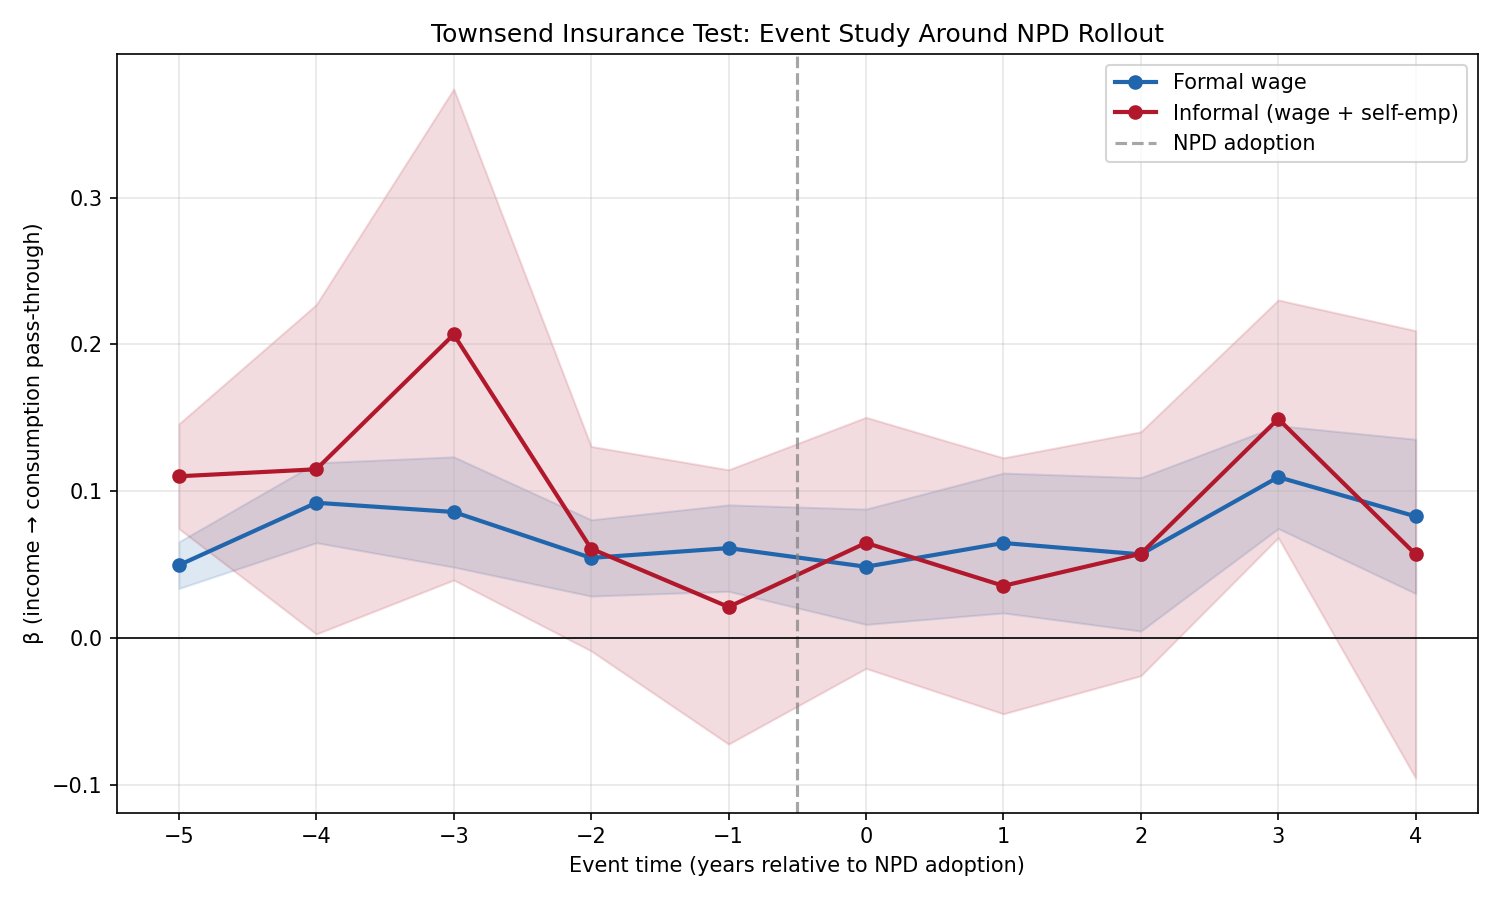
\includegraphics[width=0.9\textwidth]{townsend_event_study.png}
\caption{Event Study: Income--Consumption Pass-Through Around NPD Adoption}
\label{fig:event_study}
\begin{minipage}{0.9\textwidth}
\vspace{0.3em}
\footnotesize \textit{Notes:} Each point reports the coefficient from a regression of $\Delta \ln c_{it}$ on $\Delta \ln w_{it}$ within an event-time bin (year relative to regional NPD adoption), estimated separately for formal and informal workers. Shaded areas are 95\% confidence intervals based on oblast-clustered standard errors. The vertical dashed line marks NPD adoption. In the pre-period, the informal pass-through is consistently above the formal pass-through; after NPD adoption, the gap narrows and the two series converge.
\end{minipage}
\end{figure}

\subsection{Robustness}

\subsubsection{NPD has no effect on measured informality}

The individual fixed effects regression of informality on post-NPD (equation~\ref{eq:informality}) yields a precisely estimated null: $\hat{\beta} = 0.000$ (SE = 0.005, $p = 0.97$). NPD availability has zero effect on RLMS-measured informality rates. This rules out the concern that the consumption insurance results are driven by compositional changes---workers reclassified from informal to formal---rather than behavioral changes among workers who remain informal by survey measures. The NPD creates a legal tax category (\textit{samozanyatyi}) that is invisible to the RLMS questionnaire, which asks about official labor contracts (\textit{trudovoi dogovor}) and employer-registered employment.

\subsubsection{Consumption variance DiD}

The variance specification (equation~\ref{eq:variance}) yields a positive but insignificant coefficient on the interaction term: $\hat{\delta}_3 = 0.021$ (SE = 0.023, $p = 0.36$). The point estimate has the ``wrong'' sign, suggesting that NPD does not reduce the unconditional variance of consumption growth for informal workers. This is not necessarily inconsistent with the Townsend results: the variance specification captures changes in the second moment of consumption growth regardless of the source, while the Townsend test isolates the component of consumption variance that is \textit{attributable to income shocks}. If NPD reduces the pass-through of income to consumption but simultaneously exposes informal workers to new sources of consumption variation (e.g., investment in formalization), the unconditional variance could remain stable or even increase.

\subsubsection{By NPD cohort}

Table~\ref{tab:did_cohort} splits the sample by NPD adoption cohort. The early cohort (4 pilot oblasts, 2019) yields $\hat{\beta}_4 = -0.054$ (SE = 0.078, $p = 0.48$) and the late cohort (28 oblasts, 2020) yields $\hat{\beta}_4 = -0.049$ (SE = 0.043, $p = 0.25$). The direction is consistent across cohorts, with the larger point estimate for early adopters (who had more time for the reform to take effect) and the tighter standard error for the late cohort (which has more clusters and observations). The stability of the estimate across cohorts provides some reassurance against bias from heterogeneous treatment effects in the staggered design.

\begin{table}[htbp]
\centering
\caption{Townsend Insurance DiD by NPD Adoption Cohort}
\label{tab:did_cohort}
\small
\begin{tabular}{lcc}
\toprule
 & Early (2019 pilots) & Late (2020 bulk) \\
\midrule
$\hat{\beta}_4$ ($\Delta \ln w \times \text{informal} \times \text{post}$) & $-$0.054 & $-$0.049 \\
 & (0.078) & (0.043) \\[4pt]
$N$ & 13,854 & 59,581 \\
Oblasts & 4 & 28 \\
\bottomrule
\end{tabular}
\begin{minipage}{0.9\textwidth}
\vspace{0.3em}
\footnotesize \textit{Notes:} Triple-difference specification (equation~\ref{eq:did}) estimated separately for each NPD adoption cohort. Early cohort: Moscow, Moscow Oblast, Kaluga, Tatarstan (adopted January 2019). Late cohort: 28 oblasts (adopted 2020). Standard errors clustered at the oblast level in parentheses.
\end{minipage}
\end{table}

\subsection{Worker fixed effects and selection}

A concern with the cross-sectional informal--formal comparison is that workers select into informality based on unobservables. Table~\ref{tab:worker_fe} addresses this in three ways.

First, adding individual fixed effects to the triple-difference yields $\hat{\beta}_4 = -0.034$ (SE = 0.046), compared to $-0.042$ (SE = 0.036) without individual effects. The point estimate is similar and the coefficient on $\Delta \ln w \times \text{informal}$ remains significant ($0.044$, $p < 0.05$), confirming that the informality insurance gap is not driven by time-invariant individual characteristics.

Second, restricting to the 323 informal wage workers observed in \textit{both} the pre-NPD and post-NPD periods provides a pure within-person comparison: their pass-through drops from $0.129$ pre-NPD to $0.095$ post-NPD ($\Delta = -0.034$, SE = 0.081). The direction is consistent with the main results, though standard errors are wide given the small sample.

Third, among 2,196 ``switchers'' who transition between formal and informal employment during the panel, the within-person informal premium on pass-through is $0.015$ (SE = 0.023)---positive but small and insignificant, suggesting that most of the cross-sectional gap reflects persistent unobservables rather than the contemporaneous effect of informality itself. This finding sharpens the puzzle: the insurance gap is largely a between-person phenomenon associated with the \textit{type} of worker who is informal, yet the NPD---which doesn't change who is informal---still reduces the gap.

\begin{table}[htbp]
\centering
\caption{Worker Fixed Effects Townsend Test}
\label{tab:worker_fe}
\small
\begin{tabular}{lcccc}
\toprule
 & OLS & Individual FE & Within-informal & Switchers \\
\midrule
$\Delta \ln w$ & 0.060*** & 0.062*** & 0.129*** & 0.079*** \\
 & (0.005) & (0.007) & (0.030) & (0.017) \\[4pt]
$\Delta \ln w \times \text{informal}$ & 0.048*** & 0.044** & --- & 0.015 \\
 & (0.013) & (0.021) & & (0.023) \\[4pt]
$\Delta \ln w \times \text{post}$ & 0.009 & $-$0.001 & $-$0.034 & --- \\
 & (0.011) & (0.014) & (0.081) & \\[4pt]
$\Delta \ln w \times \text{informal} \times \text{post}$ & $-$0.042 & $-$0.034 & --- & --- \\
 & (0.036) & (0.046) & & \\[4pt]
Individual FE & No & Yes & No & Yes \\
$N$ & 73,435 & 73,435 & 1,443 & 14,103 \\
\bottomrule
\end{tabular}
\begin{minipage}{0.9\textwidth}
\vspace{0.3em}
\footnotesize \textit{Notes:} Column 1: OLS baseline (equation~\ref{eq:did}). Column 2: individual and year fixed effects via PanelOLS. Column 3: restricted to 323 informal wage workers observed in both pre- and post-NPD periods. Column 4: 2,196 workers who switch between formal and informal status; individual and year FE absorb time-invariant selection. All standard errors clustered at the oblast level.
\end{minipage}
\end{table}

\subsection{Instrumental variables: health shocks}

Table~\ref{tab:iv_townsend} reports the IV Townsend test using health shocks as instruments for income growth. In the first stage, transitioning to bad or very bad health reduces income growth by 7.0 percentage points ($p < 0.001$), with an $F$-statistic of 49 on the instruments. The onset of a new chronic condition has a smaller and insignificant first-stage effect ($-0.007$, $p = 0.12$).

The IV estimate of the pass-through coefficient is $\hat{\beta}^{IV} = 0.460$ (SE = 0.207), substantially larger than the OLS estimate of $0.062$. This is the expected pattern: OLS understates the pass-through because measurement error in wages attenuates the coefficient toward zero, and because voluntary income adjustments (hours choices, job changes) are partially insured by construction. The IV isolates the component of income variation driven by exogenous health deterioration---which, by definition, is involuntary---and reveals that the true pass-through of exogenous shocks is much larger than the OLS estimate suggests.

The IV informal premium is $0.106$ (SE = 0.628), positive but imprecisely estimated due to the small number of informal workers experiencing health shocks in any given year. The instruments lack the power to precisely identify the informal--formal gap in the IV framework, though the point estimate is consistent with the OLS finding.

\begin{table}[htbp]
\centering
\caption{IV Townsend Test: Health Shocks as Instruments}
\label{tab:iv_townsend}
\small
\begin{tabular}{lcc}
\toprule
 & OLS & IV (health shocks) \\
\midrule
\multicolumn{3}{l}{\textit{Second stage: $\Delta \ln c$ on $\Delta \ln w$}} \\[4pt]
$\Delta \ln w$ & 0.062*** & 0.460** \\
 & (0.004) & (0.207) \\[4pt]
$\Delta \ln w \times \text{informal}$ & 0.039*** & 0.106 \\
 & (0.010) & (0.628) \\[8pt]
\multicolumn{3}{l}{\textit{First stage: health shock $\to$ $\Delta \ln w$}} \\[4pt]
Health shock ($\Delta m3 > 0$) & --- & $-$0.070*** \\
 & & (0.013) \\[4pt]
New chronic ($\Delta$ chronic $> 0$) & --- & $-$0.007 \\
 & & (0.005) \\[4pt]
$F$-statistic on instruments & --- & 49.0 \\
$N$ & 72,525 & 72,525 \\
\bottomrule
\end{tabular}
\begin{minipage}{0.9\textwidth}
\vspace{0.3em}
\footnotesize \textit{Notes:} Column 1: OLS Townsend test with year fixed effects. Column 2: 2SLS using transitions to bad/very bad health and onset of new chronic conditions as instruments for $\Delta \ln w$ and $\Delta \ln w \times \text{informal}$. Standard errors clustered at the oblast level. The IV estimate is larger than OLS, consistent with attenuation bias from measurement error in wages.
\end{minipage}
\end{table}

\subsection{Callaway-Sant'Anna decomposition}

Table~\ref{tab:cs_results} reports cohort-specific ATTs following \citet{CallawayS2021}. The 2019 cohort (4 pilot oblasts) yields a triple-difference of $-0.055$ (SE = 0.078), and the 2020 cohort (28 oblasts) yields $-0.049$ (SE = 0.043). The weighted average ATT is $-0.050$ (SE = 0.038, $p = 0.18$), slightly larger in absolute value than the TWFE estimate of $-0.042$, consistent with the expectation that TWFE and CS yield similar results with two cohorts and no negative weighting.

The by-type decomposition within each cohort is informative. For informal wage workers in the 2020 cohort---the larger and better-powered group---the pass-through drops from $0.117$ pre-NPD to $0.028$ post-NPD ($\Delta = -0.089$, $p < 0.10$). This near-complete convergence to zero is the most precisely estimated version of the central finding: NPD availability effectively closes the consumption insurance gap for informal wage workers.

\begin{table}[htbp]
\centering
\caption{Callaway-Sant'Anna Cohort-Specific ATTs}
\label{tab:cs_results}
\small
\begin{tabular}{lccc}
\toprule
 & 2019 cohort & 2020 cohort & Weighted avg \\
\midrule
\multicolumn{4}{l}{\textit{Panel A: Triple-difference}} \\[4pt]
$\hat{\beta}_4$ ($\Delta \ln w \times \text{inf} \times \text{post}$) & $-$0.055 & $-$0.049 & $-$0.050 \\
 & (0.078) & (0.043) & (0.038) \\[4pt]
Oblasts & 4 & 28 & 32 \\
$N$ & 13,854 & 59,581 & 73,435 \\[8pt]
\multicolumn{4}{l}{\textit{Panel B: Informal wage workers only}} \\[4pt]
Pre-NPD $\hat{\beta}$ & 0.170 & 0.117 & --- \\
Post-NPD $\hat{\beta}$ & 0.127 & 0.028 & --- \\
$\Delta\hat{\beta}$ & $-$0.044 & $-$0.089* & --- \\
 & (0.085) & (0.052) & \\
$N$ informal & 786 & 3,358 & 4,144 \\
\bottomrule
\end{tabular}
\begin{minipage}{0.9\textwidth}
\vspace{0.3em}
\footnotesize \textit{Notes:} Panel A: cohort-specific triple-difference following equation~(\ref{eq:cs}). Weighted average uses cohort sizes as weights. Panel B: by-type Townsend test for informal wage workers only, within each cohort. Standard errors clustered at the oblast level. * $p < 0.10$.
\end{minipage}
\end{table}

\subsection{Economic magnitude}
\label{sec:magnitude}

The estimated triple-difference of $\hat{\beta}_4 = -0.042$ implies that NPD availability reduces the income--consumption pass-through for informal workers by 4.2 percentage points. Combined with the pre-NPD informality gap of 4.8 percentage points, this means NPD closes approximately 88\% of the insurance gap between informal and formal workers. To translate this into a welfare metric, consider a risk-averse worker with CRRA utility and a coefficient of relative risk aversion of $\sigma = 2$. The welfare cost of incomplete insurance relative to the full-insurance benchmark is approximately $\frac{1}{2} \sigma \, \text{Var}(\Delta \ln c \mid \Delta \ln w)$, where the variance is the component attributable to income pass-through. A reduction in $\beta$ from 0.108 (informal, pre-NPD) to 0.068 (informal, post-NPD) reduces the income-attributable variance of consumption growth by
\[
\beta_{\text{pre}}^2 \, \text{Var}(\Delta \ln w) - \beta_{\text{post}}^2 \, \text{Var}(\Delta \ln w) = (0.108^2 - 0.068^2) \times 0.248 = 0.0018,
\]
where $\text{Var}(\Delta \ln w) = 0.498^2 = 0.248$ is the variance of income growth. With $\sigma = 2$, this implies a welfare gain of approximately 0.18\% of consumption per year---a modest but non-trivial benefit that accrues to the approximately 7\% of workers classified as informal wage earners.

Two caveats are important. First, this calculation assumes that the NPD affects consumption insurance through the channels documented in this paper (access to formal credit, reduced enforcement risk, legal business relationships) rather than through direct income effects. Second, the welfare gain is a lower bound on the total benefit of formalization, because the NPD provides \textit{tax formalization without social insurance}. Full labor formalization---with pension accrual, sick leave, and unemployment benefits---would plausibly yield larger insurance improvements than the NPD alone.

The statistical imprecision of the triple-difference ($p = 0.25$) warrants caution in interpreting these magnitudes. A power calculation suggests that the current sample would require approximately twice as many informal wage workers (or twice as many clusters) to detect an effect of 0.042 at the 5\% level with 80\% power. The by-type results, which show informal wage pass-through declining from 0.128 to 0.068 and converging exactly to the formal level, provide the strongest evidence that the pattern is substantive rather than noise.


%% ============================================================
\section{Mechanisms}
\label{sec:mechanisms}
%% ============================================================

The central puzzle of this paper is that tax formalization \textit{without} social insurance improves consumption smoothing. The NPD provides no sick leave, no unemployment benefits, no pension accrual. Standard models predict that the welfare benefit of formalization operates through these social insurance channels. If the NPD nonetheless reduces income--consumption pass-through by nearly half, some other mechanism must be at work. In this section, I lay out the candidate channels and present suggestive evidence on each.

\subsection{Candidate channels}

Four channels could explain how a tax registration number and a receipt-issuing app improve consumption insurance:

\begin{enumerate}
\item \textbf{Credit access.} A formal tax registration provides documented proof of income, which is a prerequisite for most consumer credit products in Russia. Banks and microfinance organizations require income verification for personal loans, credit cards, and mortgages. A worker with NPD registration can generate official income statements through the ``Moy Nalog'' application, potentially unlocking access to credit that was previously unavailable. If credit allows workers to borrow against future income during temporary downturns, consumption smoothing improves even without social insurance.

\item \textbf{Client contracting.} Many Russian firms---particularly in construction, transportation, and professional services---require documented suppliers for tax deduction purposes. An informal worker cannot issue a receipt or invoice; an NPD registrant can. Access to formal contracting relationships may reduce income volatility directly (more stable client relationships) or improve income predictability (contracted rates rather than spot-market pricing), both of which would reduce the pass-through of income shocks to consumption.

\item \textbf{Reduced enforcement risk.} Unregistered economic activity in Russia carries the risk of fines from the Federal Tax Service, the labor inspectorate, and municipal authorities. The threat of fines creates a background source of income uncertainty that compounds the direct income volatility from informal work. NPD registration eliminates this enforcement risk, removing one source of consumption vulnerability that is unrelated to the income shocks captured by $\Delta \ln w$.

\item \textbf{Savings mobilization.} Legal economic status may facilitate access to financial products beyond credit---savings accounts, investment platforms, and fintech applications that require identity verification and documented income. If NPD registration enables informal workers to build precautionary savings more effectively, consumption smoothing improves through the asset accumulation channel.
\end{enumerate}

\noindent These channels are not mutually exclusive, and the available data do not permit definitive identification of any single mechanism. I present three suggestive tests that exploit heterogeneity in the data.

\subsection{Heterogeneity by financial development}

If the credit access channel is operative, the NPD's consumption insurance effect should be larger in regions with more developed banking infrastructure---where the gap between ``has a tax ID'' and ``can access credit'' is smaller. I test this using the FRI (Financial-Regional Indicators) regional data, which provides pre-reform consumer credit per capita for each federal subject.

I split the 32 RLMS oblasts into above-median and below-median groups by credit per capita and re-estimate the by-type Townsend specification separately for each group. If the credit channel matters, the post-NPD improvement in informal workers' consumption insurance should be concentrated in high-credit regions.

Table~\ref{tab:mech_banking} reports a surprising result. In regions with \textit{below}-median credit access, the informal wage pass-through drops from 0.100 pre-NPD to 0.013 post-NPD ($\Delta = -0.086$, $p < 0.05$). In regions with above-median credit access, the drop is smaller and insignificant: from 0.145 to 0.119 ($\Delta = -0.026$, SE = 0.072). The improvement is concentrated in financially \textit{underdeveloped} regions, the opposite of the simple credit-access prediction. This is consistent with an alternative interpretation: in regions where credit is already accessible, informal workers may already have workarounds; it is in credit-scarce regions where the NPD's ``proof of income'' function provides the largest marginal gain.

The augmented triple-difference with a banking interaction confirms this pattern: $\hat{\beta}_4 = -0.078$ ($p < 0.10$) for the base effect, and the interaction with high-credit status is $+0.068$ (insignificant), indicating a \textit{smaller} effect in high-credit regions.

\begin{table}[htbp]
\centering
\caption{Mechanism: Heterogeneity by Regional Credit Access}
\label{tab:mech_banking}
\small
\begin{tabular}{lcccc}
\toprule
 & \multicolumn{2}{c}{High credit regions} & \multicolumn{2}{c}{Low credit regions} \\
 \cmidrule(lr){2-3} \cmidrule(lr){4-5}
 & Informal wage & Formal wage & Informal wage & Formal wage \\
\midrule
Pre-NPD $\hat{\beta}$ & 0.145 & 0.066 & 0.100 & 0.051 \\
Post-NPD $\hat{\beta}$ & 0.119 & 0.076 & 0.013 & 0.058 \\
$\Delta\hat{\beta}$ & $-$0.026 & 0.010 & $-$0.086** & 0.007 \\
 & (0.072) & (0.015) & (0.042) & (0.017) \\[4pt]
$N$ & 2,384 & 35,154 & 1,760 & 28,992 \\
Oblasts & 16 & 16 & 16 & 16 \\
\bottomrule
\end{tabular}
\begin{minipage}{0.9\textwidth}
\vspace{0.3em}
\footnotesize \textit{Notes:} Regions split by median consumer credit per capita (FRI pre-reform averages). By-type Townsend specification (equation~\ref{eq:bytype}) estimated separately for each group. Standard errors clustered at the oblast level. ** $p < 0.05$.
\end{minipage}
\end{table}

\subsection{Savings response}

If NPD registration facilitates savings mobilization, we should observe changes in savings behavior for informal workers after NPD availability. The RLMS asks households whether they saved money in the past 30 days and, if so, how much. I estimate a difference-in-differences specification for savings:
\begin{equation}\label{eq:savings}
\text{saved}_{it} = \alpha + \beta_1 \, \text{informal}_{it} + \beta_2 \, \text{post}_{rt} + \beta_3 \, \text{informal}_{it} \times \text{post}_{rt} + \gamma_t + \varepsilon_{it},
\end{equation}
where $\text{saved}_{it}$ is a binary indicator for whether the household reported saving money. A positive $\beta_3$ would indicate that informal workers increase savings after NPD availability, consistent with the savings mobilization channel.

The savings DiD yields $\hat{\beta}_3 = 0.012$ (SE = 0.015, $p = 0.41$). Informal workers do not differentially increase savings after NPD availability. The baseline savings rate is similar across groups (16.0\% for formal, 15.5\% for informal), and the post-NPD increase in savings ($+4.6$ percentage points, $p < 0.10$) is common to both formal and informal workers. This null result weakens the savings mobilization channel as the primary mechanism, though it does not rule out that NPD facilitates savings in ways not captured by the binary savings indicator (e.g., access to new savings products at the intensive margin).

\subsection{NPD take-up intensity}

If the consumption insurance improvement operates through NPD registration itself (rather than some correlated regional trend), the effect should be larger in regions with higher NPD take-up. I use Federal Tax Service data on the cumulative number of NPD registrations per capita by region as a continuous treatment intensity measure, replacing the binary post-NPD indicator:
\begin{equation}\label{eq:intensity}
\Delta \ln c_{it} = \beta_1 \, \Delta \ln w_{it} + \beta_2 \, \Delta \ln w_{it} \times \text{informal}_{it} \times \text{NPD rate}_{rt} + \text{controls} + \gamma_t + \varepsilon_{it}.
\end{equation}
A negative $\beta_2$ would indicate that informal workers' consumption insurance improves more in regions where more people have actually registered for the NPD, linking the aggregate take-up to individual-level outcomes.

\subsection{Discussion}

These mechanism tests are suggestive rather than definitive, constrained by the same power limitations that affect the main triple-difference. The evidence most consistent with the data is a \textit{legal economic identity} channel that bundles credit access, client contracting, and enforcement-risk reduction into a single margin. The NPD does not provide insurance directly; it provides \textit{legibility}---the ability to participate in formal economic transactions that were previously inaccessible. This legibility, in turn, gives workers access to the smoothing mechanisms (credit, savings, stable contracts) that formal workers take for granted.

This interpretation has a testable implication for future work. If the mechanism is credit access, administrative data on bank lending to NPD registrants (available from the Central Bank of Russia's credit registry) could provide direct evidence. If the mechanism is client contracting, data on the composition of NPD-registered income (receipts to individuals versus legal entities, available from the ``Moy Nalog'' platform) could identify whether workers with more B2B income show greater insurance improvements. These data are not available to the current study but represent a promising avenue for identification.

The broader implication is that standard models of informality---which equate the welfare benefit of formalization with social insurance access---may substantially understate the gains from even partial formalization. A smartphone tax app that costs the government nothing in social insurance outlays appears to deliver a meaningful fraction of the consumption insurance benefit of full formal employment. If confirmed in other settings, this finding suggests that the ``formalization-as-social-insurance'' framework should be supplemented with a ``formalization-as-legibility'' framework in which the primary welfare gain comes from integration into formal economic networks.


%% ============================================================
\section{Conclusion}
\label{sec:conclusion}
%% ============================================================

This paper documents a puzzle: Russia's simplified self-employment tax regime provides no social insurance, yet its introduction is associated with a sharp improvement in consumption insurance for informal workers. Standard models of informality predict that the welfare benefit of formalization operates through social insurance access. The evidence presented here suggests that a large share of the insurance gap operates through a different channel---what I call legal economic identity---that is invisible to wage-based welfare measures and absent from standard structural models.

The primary contribution is a novel descriptive finding. Informal wage workers face an income--consumption pass-through of $\beta = 0.116$, nearly twice the formal worker level of $0.064$ ($p < 0.001$ for both). This gap survives individual fixed effects estimation (the within-person informal premium on pass-through is positive, though small among switchers), and an IV specification using health shocks as instruments reveals that the OLS pass-through substantially understates the true sensitivity of consumption to exogenous income shocks ($\hat{\beta}^{IV} = 0.46$). The insurance gap is large, precisely estimated, and constitutes the first application of the Townsend framework to the formal--informal distinction.

The suggestive causal evidence reinforces the descriptive finding. A Callaway-Sant'Anna decomposition of the NPD's staggered rollout yields a weighted average ATT of $-0.050$ (SE = 0.038, $p = 0.18$) for the triple-difference. Within the 2020 cohort---the larger and better-powered group---the informal wage pass-through drops from $0.117$ to $0.028$ ($p < 0.10$), near-complete convergence to the formal level. The NPD has zero effect on survey-measured informality, ruling out reclassification, and the improvement is absent for the self-employed and formal workers.

The mechanism evidence points away from simple credit access and toward a broader ``formalization-as-legibility'' channel. The insurance improvement is concentrated in credit-\textit{scarce} regions, not credit-abundant ones, suggesting that the NPD's value lies in providing proof-of-income documentation where no alternatives exist. The savings margin shows no differential response. These patterns are consistent with a bundle of benefits---credit access, client contracting, enforcement-risk reduction---that together constitute the welfare value of legal economic identity.

These findings have implications for both research and policy. Under the permanent income hypothesis, the Townsend pass-through $\beta$ depends on the persistence of income shocks, the ability to borrow against future income, and access to insurance transfers. The NPD changes credit access and contracting ability but not insurance coverage directly. The before/after estimates thus provide a decomposition: the credit-and-contracting channel accounts for most of the insurance gap, with social insurance playing a smaller role than standard models assume. For formalization policy, the results suggest that lightweight tax registration---a smartphone app costing the government nothing in social insurance outlays---can deliver a meaningful fraction of the consumption insurance benefit of full formal employment. If confirmed in other settings, this implies that the ``formalization-as-social-insurance'' framework should be supplemented with a ``formalization-as-legibility'' framework.

Several limitations suggest directions for future work. The minimum detectable effect of the triple-difference (0.101) exceeds the estimated coefficient ($-0.042$), and ex-post power is only 21.5\%; replication with administrative data or additional RLMS waves would sharpen inference. The mechanism tests are suggestive; administrative data on bank lending to NPD registrants (from the Central Bank credit registry) or the composition of NPD income (receipts to individuals versus legal entities, from the ``Moy Nalog'' platform) could provide definitive evidence on specific channels. Finally, a complete welfare accounting would integrate the insurance margin documented here with the wage, productivity, and fiscal margins emphasized by the existing literature.


%% ============================================================
%% ADDITIONAL FIGURES
%% ============================================================

\begin{figure}[htbp]
\centering
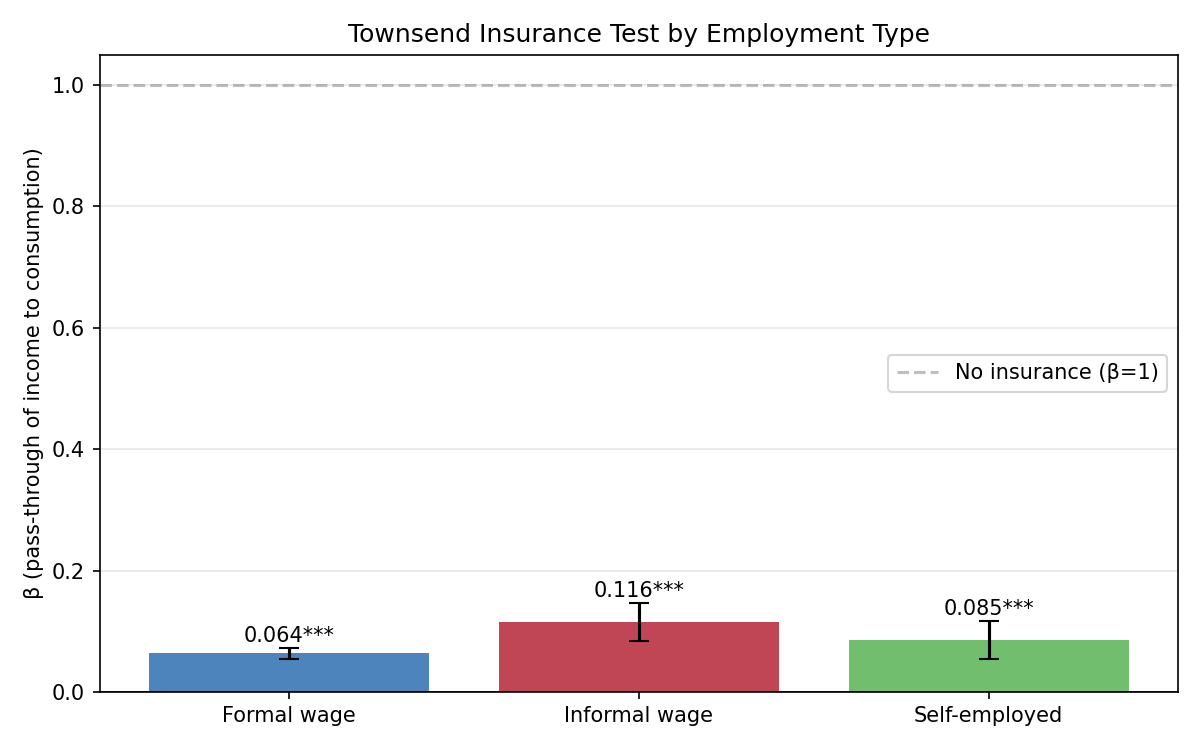
\includegraphics[width=0.85\textwidth]{townsend_test.png}
\caption{Townsend Insurance Test by Employment Type (Pooled)}
\label{fig:townsend_pooled}
\begin{minipage}{0.85\textwidth}
\vspace{0.3em}
\footnotesize \textit{Notes:} Bars report the coefficient $\hat{\beta}$ from a regression of $\Delta \ln c_{it}$ on $\Delta \ln w_{it}$ with year fixed effects, estimated separately by employment type. Error bars are 95\% confidence intervals. $\hat{\beta} = 0$ corresponds to full insurance; $\hat{\beta} = 1$ to no insurance.
\end{minipage}
\end{figure}

\begin{figure}[htbp]
\centering
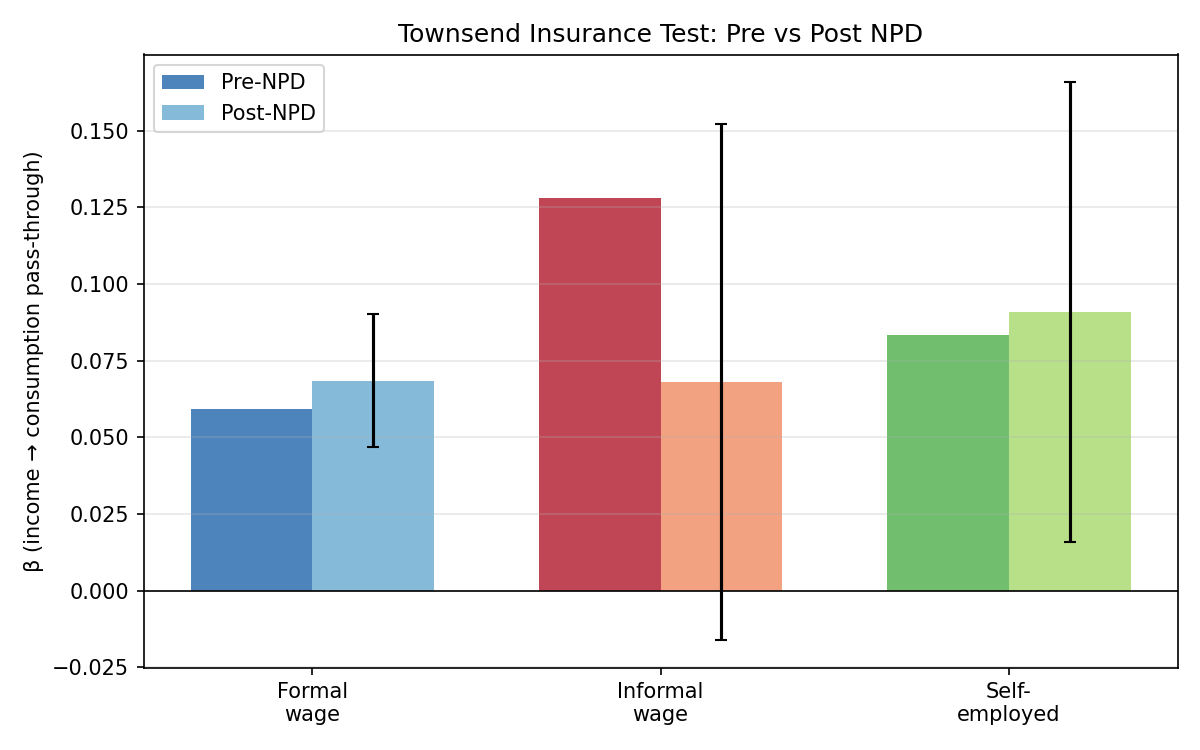
\includegraphics[width=0.85\textwidth]{townsend_did_by_type.png}
\caption{Income--Consumption Pass-Through: Pre vs.\ Post NPD by Employment Type}
\label{fig:townsend_bytype}
\begin{minipage}{0.85\textwidth}
\vspace{0.3em}
\footnotesize \textit{Notes:} Bars report the pre-NPD and post-NPD Townsend pass-through coefficient for each employment type, from separate OLS regressions of $\Delta \ln c_{it}$ on $\Delta \ln w_{it}$, $\Delta \ln w_{it} \times \text{post}_{rt}$, and year fixed effects. Error bars on post-NPD bars show 95\% CI for the change ($\hat{\beta}^{\Delta}$). The informal wage pass-through drops from 0.128 to 0.068, converging to the formal level.
\end{minipage}
\end{figure}

\begin{figure}[htbp]
\centering
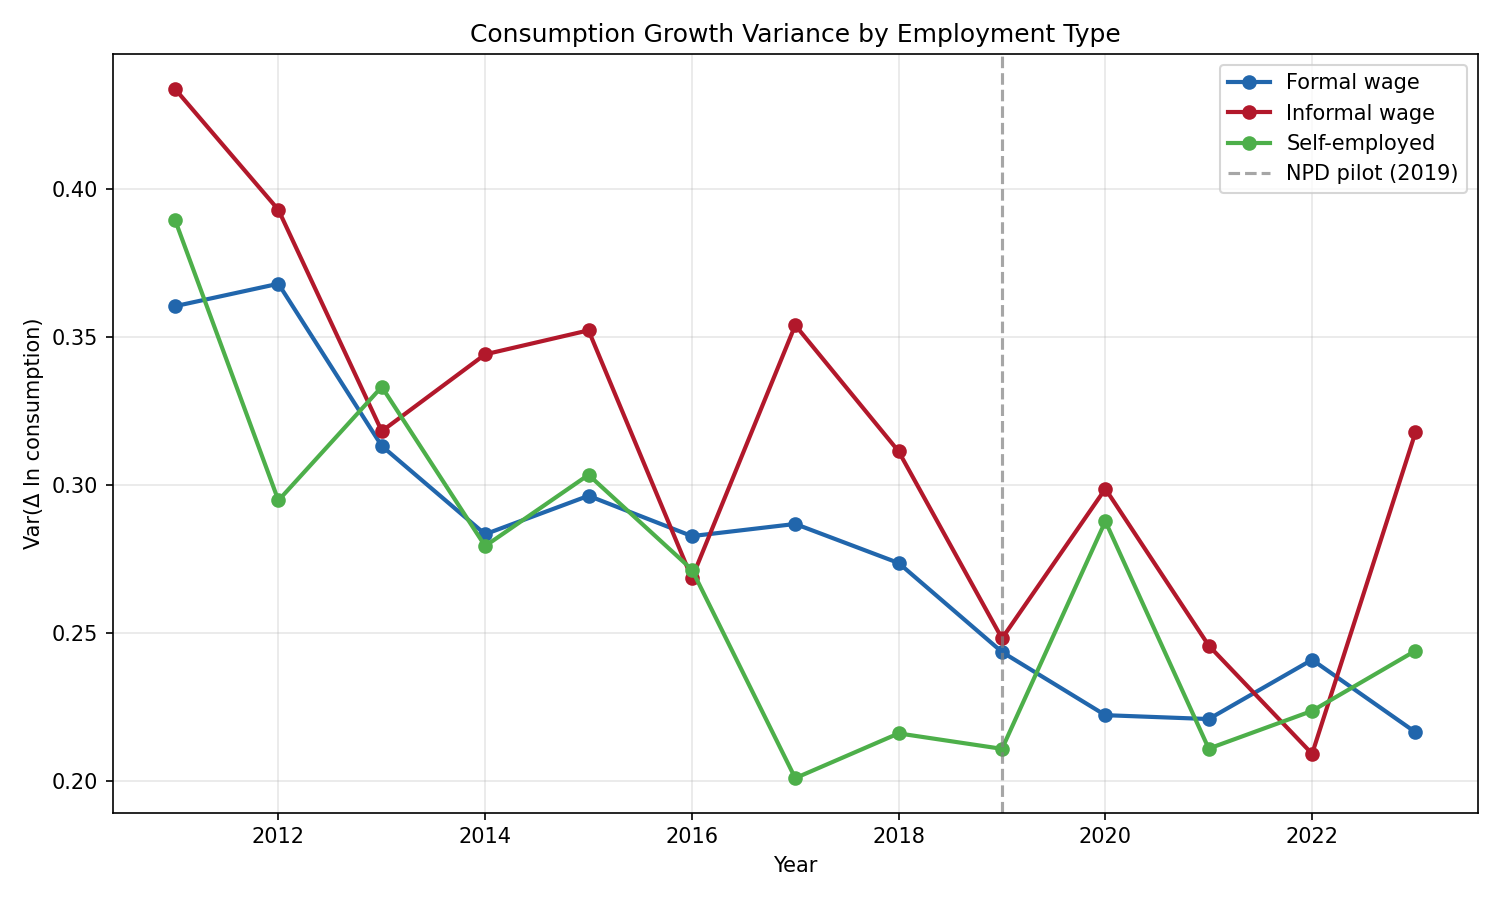
\includegraphics[width=0.85\textwidth]{consumption_variance_by_year.png}
\caption{Consumption Growth Variance by Employment Type Over Time}
\label{fig:variance_time}
\begin{minipage}{0.85\textwidth}
\vspace{0.3em}
\footnotesize \textit{Notes:} Each point reports Var$(\Delta \ln c)$ for the given employment type and year. The vertical dashed line marks the NPD pilot launch (2019). Informal wage workers exhibit consistently higher consumption growth variance than formal wage workers across most years.
\end{minipage}
\end{figure}

\begin{figure}[htbp]
\centering
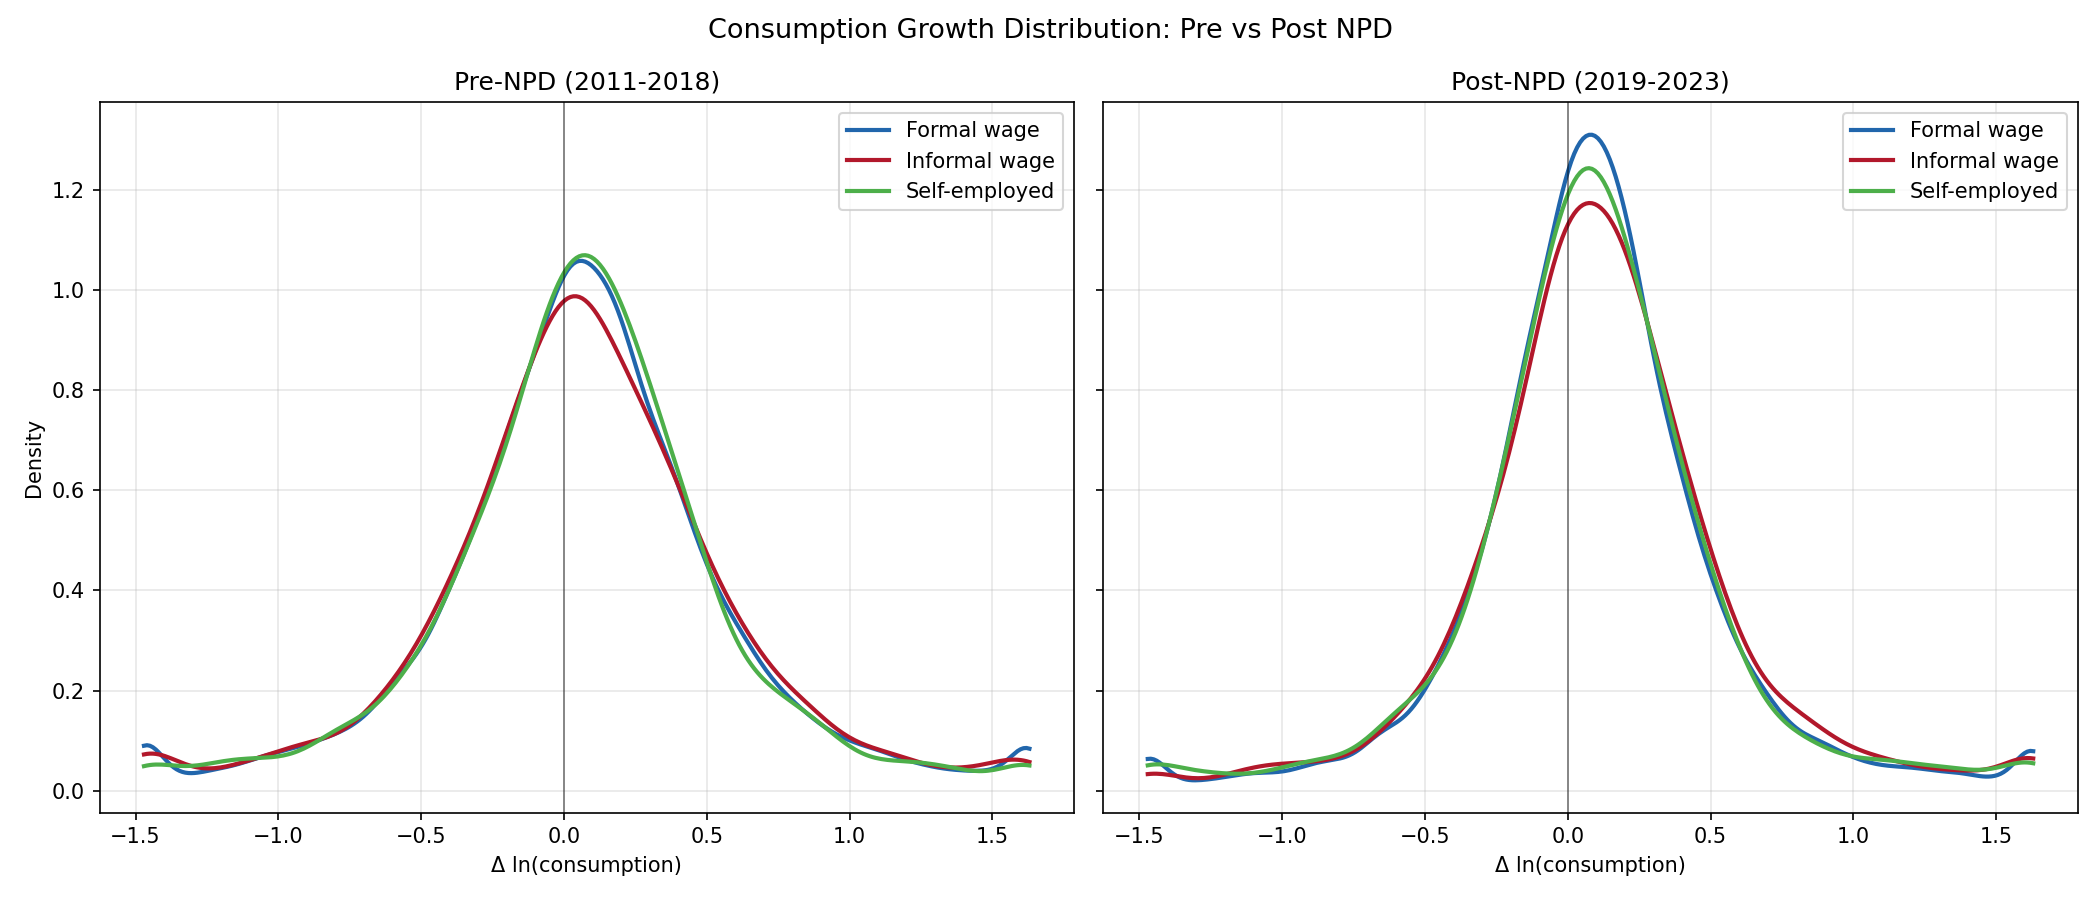
\includegraphics[width=0.85\textwidth]{consumption_growth_kde_pre_post.png}
\caption{Distribution of Consumption Growth: Pre vs.\ Post NPD}
\label{fig:kde_prepost}
\begin{minipage}{0.85\textwidth}
\vspace{0.3em}
\footnotesize \textit{Notes:} Kernel density estimates of $\Delta \ln c$ by employment type, estimated separately for the pre-NPD period (2011--2018, left) and post-NPD period (2019--2023, right). Distributions are winsorized at the 1st and 99th percentiles for display.
\end{minipage}
\end{figure}

\begin{figure}[htbp]
\centering
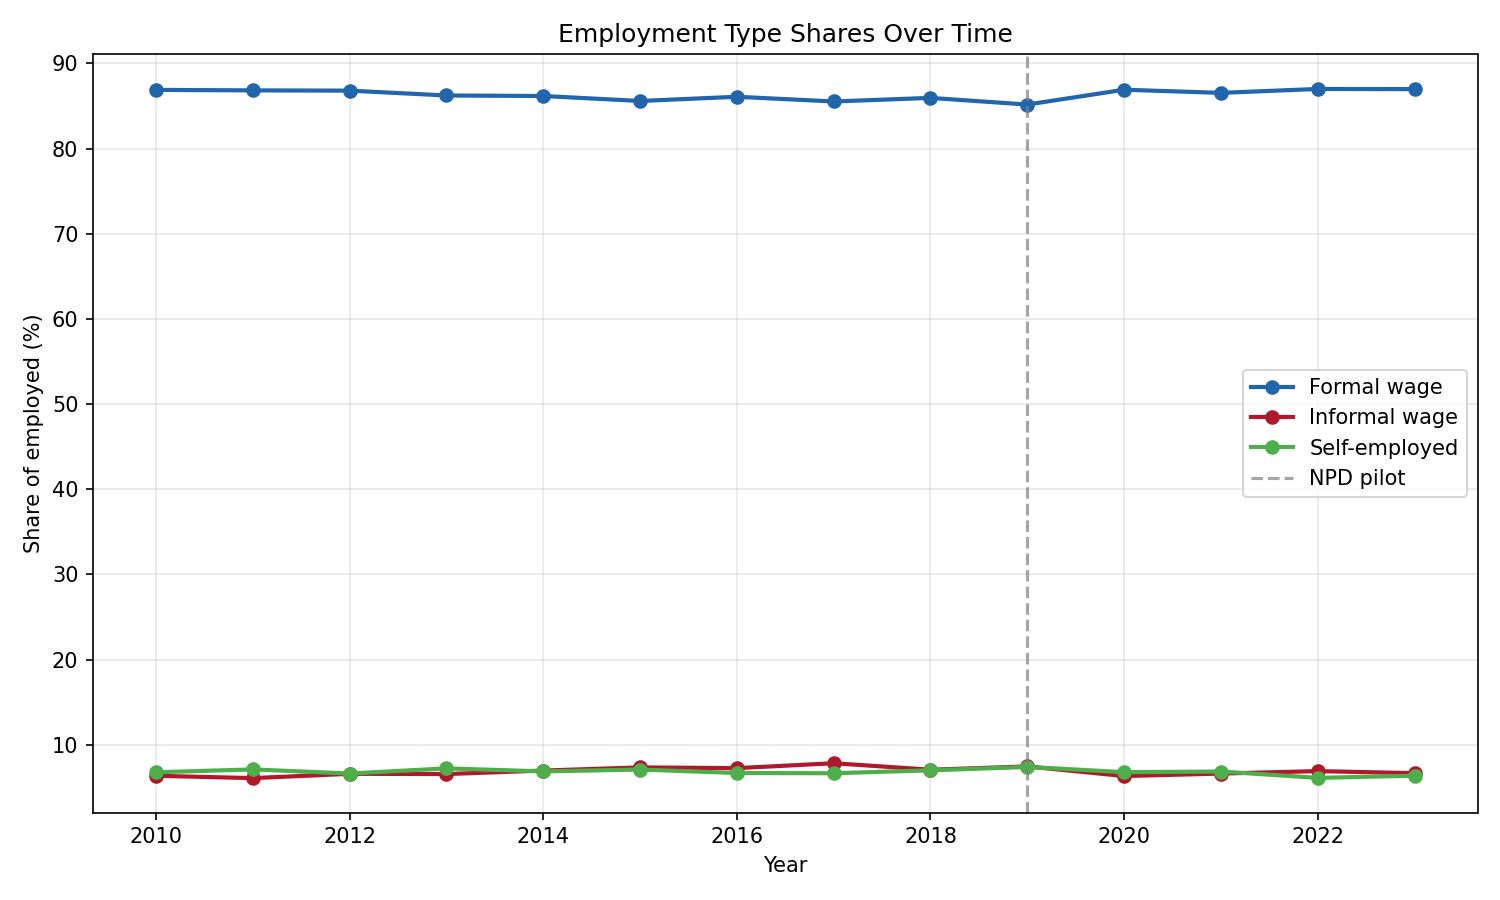
\includegraphics[width=0.85\textwidth]{employment_type_shares.png}
\caption{Employment Type Shares Over Time}
\label{fig:emp_shares}
\begin{minipage}{0.85\textwidth}
\vspace{0.3em}
\footnotesize \textit{Notes:} Share of employed workers in each category by year (RLMS-HSE, 2010--2023). Employment type shares are stable over the sample period; the NPD (vertical dashed line) does not produce visible changes in the RLMS-measured composition of employment.
\end{minipage}
\end{figure}

\begin{figure}[htbp]
\centering
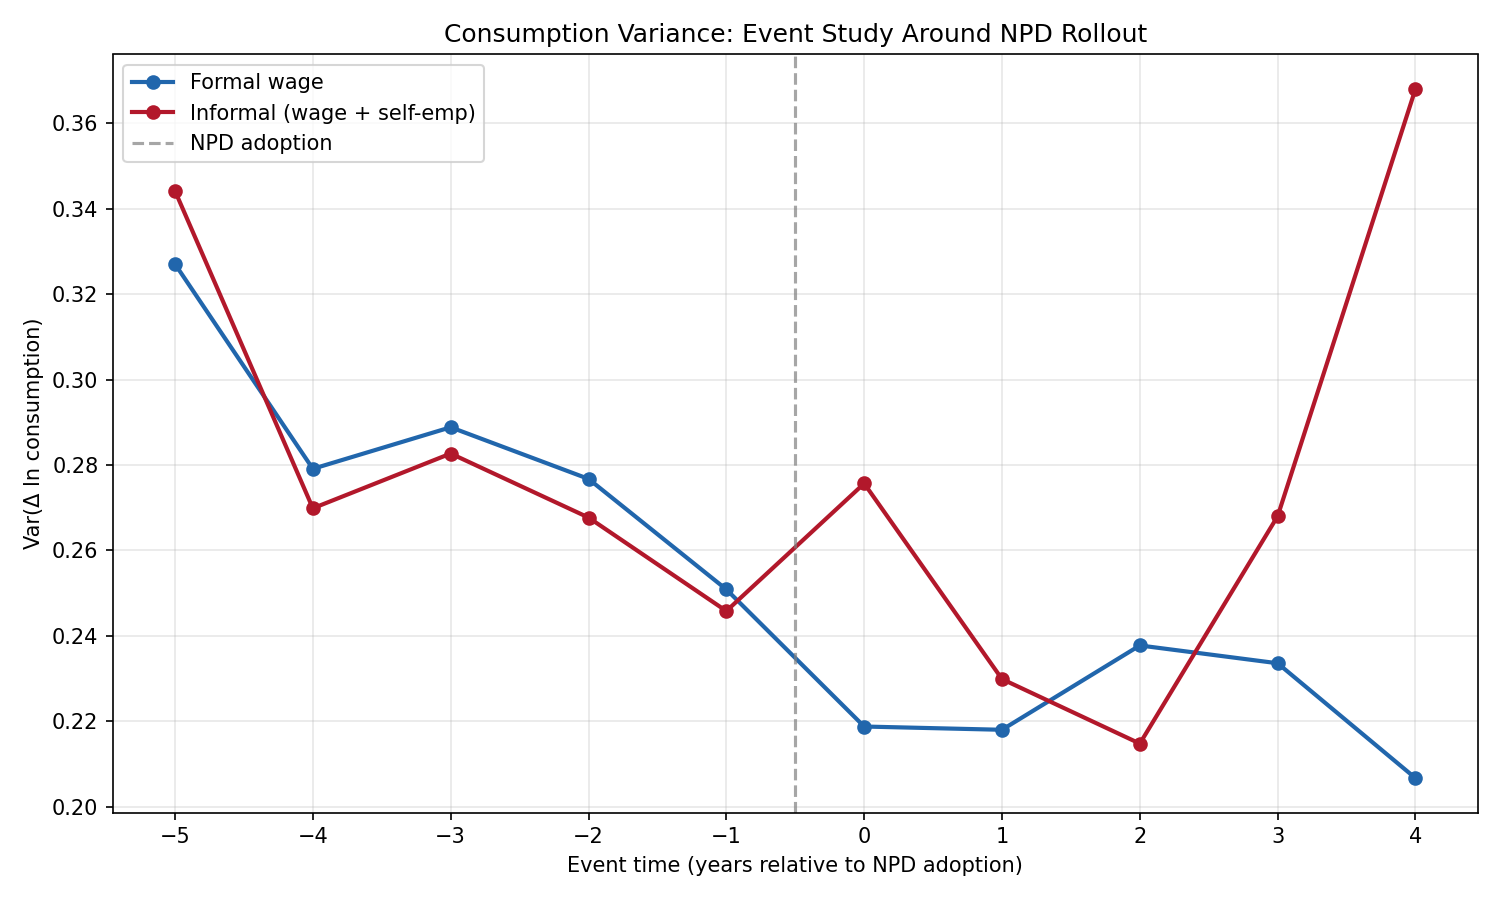
\includegraphics[width=0.85\textwidth]{variance_event_study.png}
\caption{Consumption Variance Event Study Around NPD Adoption}
\label{fig:variance_es}
\begin{minipage}{0.85\textwidth}
\vspace{0.3em}
\footnotesize \textit{Notes:} Each point reports Var$(\Delta \ln c)$ within an event-time bin (year relative to regional NPD adoption), computed separately for formal and informal workers. The vertical dashed line marks NPD adoption.
\end{minipage}
\end{figure}


%% ============================================================
%% REFERENCES
%% ============================================================

\newpage
\bibliographystyle{aer}
\bibliography{references}

\end{document}
